\documentclass[]{elsarticle} %review=doublespace preprint=single 5p=2 column
%%% Begin My package additions %%%%%%%%%%%%%%%%%%%
\usepackage[hyphens]{url}

  \journal{Some Journal} % Sets Journal name


\usepackage{lineno} % add

\usepackage{graphicx}
%%%%%%%%%%%%%%%% end my additions to header

\usepackage[T1]{fontenc}
\usepackage{lmodern}
\usepackage{amssymb,amsmath}
\usepackage{ifxetex,ifluatex}
\usepackage{fixltx2e} % provides \textsubscript
% use upquote if available, for straight quotes in verbatim environments
\IfFileExists{upquote.sty}{\usepackage{upquote}}{}
\ifnum 0\ifxetex 1\fi\ifluatex 1\fi=0 % if pdftex
  \usepackage[utf8]{inputenc}
\else % if luatex or xelatex
  \usepackage{fontspec}
  \ifxetex
    \usepackage{xltxtra,xunicode}
  \fi
  \defaultfontfeatures{Mapping=tex-text,Scale=MatchLowercase}
  \newcommand{\euro}{€}
\fi
% use microtype if available
\IfFileExists{microtype.sty}{\usepackage{microtype}}{}
\bibliographystyle{elsarticle-harv}
\ifxetex
  \usepackage[setpagesize=false, % page size defined by xetex
              unicode=false, % unicode breaks when used with xetex
              xetex]{hyperref}
\else
  \usepackage[unicode=true]{hyperref}
\fi
\hypersetup{breaklinks=true,
            bookmarks=true,
            pdfauthor={},
            pdftitle={Introducing spatial availability, a singly-constrained competitive-access accessibility measure},
            colorlinks=false,
            urlcolor=blue,
            linkcolor=magenta,
            pdfborder={0 0 0}}
\urlstyle{same}  % don't use monospace font for urls

\setcounter{secnumdepth}{0}
% Pandoc toggle for numbering sections (defaults to be off)
\setcounter{secnumdepth}{0}


% tightlist command for lists without linebreak
\providecommand{\tightlist}{%
  \setlength{\itemsep}{0pt}\setlength{\parskip}{0pt}}


% Pandoc citation processing
\newlength{\cslhangindent}
\setlength{\cslhangindent}{1.5em}
\newlength{\csllabelwidth}
\setlength{\csllabelwidth}{3em}
\newlength{\cslentryspacingunit} % times entry-spacing
\setlength{\cslentryspacingunit}{\parskip}
% for Pandoc 2.8 to 2.10.1
\newenvironment{cslreferences}%
  {}%
  {\par}
% For Pandoc 2.11+
\newenvironment{CSLReferences}[2] % #1 hanging-ident, #2 entry spacing
 {% don't indent paragraphs
  \setlength{\parindent}{0pt}
  % turn on hanging indent if param 1 is 1
  \ifodd #1
  \let\oldpar\par
  \def\par{\hangindent=\cslhangindent\oldpar}
  \fi
  % set entry spacing
  \setlength{\parskip}{#2\cslentryspacingunit}
 }%
 {}
\usepackage{calc}
\newcommand{\CSLBlock}[1]{#1\hfill\break}
\newcommand{\CSLLeftMargin}[1]{\parbox[t]{\csllabelwidth}{#1}}
\newcommand{\CSLRightInline}[1]{\parbox[t]{\linewidth - \csllabelwidth}{#1}\break}
\newcommand{\CSLIndent}[1]{\hspace{\cslhangindent}#1}

\usepackage[font=small,skip=0pt]{caption}
\usepackage{booktabs}
\usepackage{longtable}
\usepackage{array}
\usepackage{multirow}
\usepackage{wrapfig}
\usepackage{float}
\usepackage{colortbl}
\usepackage{pdflscape}
\usepackage{tabu}
\usepackage{threeparttable}
\usepackage{threeparttablex}
\usepackage[normalem]{ulem}
\usepackage{makecell}
\usepackage{xcolor}



\begin{document}


\begin{frontmatter}

  \title{Introducing spatial availability, a singly-constrained
competitive-access accessibility measure}
      
  \begin{abstract}
  Accessibility measures are widely used in transportation, urban and
  healthcare planning, among other applications. These measures are
  weighted sums of the opportunities that can be reached given the cost
  of movement and are estimates of the potential for spatial
  interaction. These measures are useful in understanding spatial
  structure, but they do not properly account for competition due to
  multiple counting of opportunities. This leads to interpretability
  issues, as noted in recent research on balanced floating catchment
  areas (BFCA) and competitive measures of accessibility. In this paper,
  we respond to this limitation by proposing a new measure of
  \emph{spatial availability} which is calculated by imposing a single
  constraint on conventional gravity-based accessibility. This
  constraint ensures that the marginals at the destination are met and
  thus the number of opportunities are preserved across the analysis.
  Through examples, we detail the formulation of the proposed measure.
  Further, we use data from the 2016 Transportation Tomorrow Survey of
  the Greater Golden Horseshoe area in southern Ontario, Canada, to
  contrast how the conventional accessibility measure tends to
  overestimate and underestimate the number of jobs \emph{available} to
  workers. We conclude with some discussion of the possible uses of
  spatial availability and argue that, compared to conventional measures
  of accessibility, it can offer a more interpretable measure of
  opportunity access. All data and code used in this research are openly
  available which should facilitate testing by other researchers in
  their case studies.
  \end{abstract}
  
 \end{frontmatter}

\newpage

\hypertarget{introduction}{%
\section{Introduction}\label{introduction}}

Accessibility analysis is employed in transportation, geography, public
health, and many other areas, particularly as mobility-based planning is
de-emphasized in favor of access-oriented planning (Deboosere et al.,
2018; Handy, 2020; Proffitt et al., 2017; Yan, 2021). The concept of
accessibility derives its appeal from combining the spatial distribution
of opportunities and the cost of reaching them (Handy and Niemeier,
1997; Hansen, 1959).

Numerous methods for calculating accessibility have been proposed that
can be broadly organized into infrastructure-, place-, person-, and
utility-based measures (Geurs and van Wee, 2004). Of these, the
place-based family of measures is arguably the most common, capturing
the number of opportunities reachable from an origin using the
transportation network. A common type of accessibility measure is based
on the gravity model of spatial interaction; since it was first
developed by Hansen (1959) it has been widely adopted in many forms
(Arranz-López et al., 2019; e.g., Cervero et al., 2002; Geurs and van
Wee, 2004; Handy and Niemeier, 1997; Levinson, 1998; Paez, 2004).
Accessibility analysis offers a powerful tool to study the intersection
between urban structure and transportation infrastructure - however, the
interpretability of accessibility measures can be challenging (Geurs and
van Wee, 2004; Miller, 2018). A key issue is that accessibility measures
are sensitive to the number of opportunities in a region (e.g., a large
city has more jobs than a smaller city), and therefore raw values are
not easily compared across study areas (Allen and Farber, 2019).

Gravity-based accessibility indicators are in essence spatially smoothed
estimates of the total number of opportunities in a region, but the
meaning of their absolute magnitudes is unclear as they measure the
\emph{potential} for interaction (as originally defined by Wilson,
1971). For instance, in the study by Boisjoly et al. (2017), high-income
areas in Metropolitan Saul Paulo have high accessibility to employment
(e.g., X jobs per all jobs available) and low-income areas have low
accessibility to employment (e.g., Y jobs per all jobs available).
Though X or Y reflect the urban structure, and correlates identify the
relationship with employment, X and Y values can only be used within the
context of employment accessibility in Saul Paulo. For example, in study
XX which used the same employment accessibility method but for ZZ
region, the X and Y accessibility values from Saul Paul cannot be
immediately compared, but the X and Y low and high accessibility values
in ZZ reflect the region's urban structure. That being said,
decision-makers and planners find it difficult to operationalize
accessibility since it reflects urban structure and is harder to
interpret as an opportunity \emph{provision} measure. For instance, if a
small city creates 1,000 more housing units in an employment rich
neighborhood (ex., 15\% of all employment opportunities are located
within the neighbourhood (X)), could the city achieve a
provider-provision-ratio of 1.5 jobs per person? Conventional
accessibility does not reflect this ratio as a result of
\emph{inconsistent} opportunity-side and population-side counting:
opportunities are multiply counted for every population unit that can
reach them.

The inconsistent counting embedded in traditional accessibility methods
has been flagged in the context of accessibility by Merlin and Hu
(2017), Allen and Farber (2019), and Kelobonye et al. (2020), and in
Floating Catchment Area methods by Delamater (2013) and Paez et al.
(2019). A consequence is the lack of clarity on the interpretation of
the resulting values, since they tend to be inflated or deflated.
Returning to XX, the maximum job accessibility in Saul Paulo is XYZ, and
the maximum job accessibility is XY in region ZZ. This the highest count
of opportunities, weighted by associated travel costs, which a certain
population can access in the region. This maximum value, outside of
reflecting urban structure, is difficult to interpret from a
decision-maker's perspective who is deliberating planning interventions.
We believe the issue in interpretation arises since opportunities are
adjusted based on population-side travel and usage behaviour (i.e.,
travel costs, catchments, time-windows). Accessibility is not
constrained to match the number of opportunities available.

Put another way, traditional measures of accessibility do not capture
the \emph{competition} for opportunities but instead quantify access as
if every person can take every opportunity given their mobility
(Kelobonye et al., 2020; Paez et al., 2019). This \emph{inconsistency}
is not necessarily problematic if the opportunity of interest is
inexaustible, that is, if use by one unit of population does not
preclude use by another. For instance, green spaces are seldom used to
full capacity, so the presence of some population in a park does not
exclude use by others. However, inconsistent opportunity-adjustments can
be more acute when opportunities are \emph{non-divisible} or
\emph{exahustible} in the sense that, once taken, they are no longer
available to other members of the population (also discussed by Geurs
and van Wee, 2004). Examples of these types of opportunities include
jobs (e.g., when a person takes up a job, the same job cannot be taken
by anyone else) and placements at schools (e.g., once a student takes a
seat at a school, that opportunity is no longer available for another
student). Though these non-divisible opportunities can still be modelled
by conventional accessibility (e.g., ), the measure does not reflect the
\emph{spatial availability} of the opportunity.

To increase the interpretability of accessibility, researchers have
proposed several different approaches that consider congestion. These
include several approaches that first normalize the number of
opportunities available at a destination by the demand from the origin
zones and, second, sum the demand-corrected opportunities which can be
reached from the origins (e.g. Joseph and Bantock, 1984; Shen, 1998).
These advances were popularized in the family of two-step floating
catchment area (FCA) methods (Luo and Wang, 2003) that have found
widespread adoption for calculating accessibility with congestion to a
variety of opportunities such as healthcare, education, and food access
(B. Y. Chen et al., 2020; Chen, 2019; Z. Chen et al., 2020; Yang et al.,
2006; Ye et al., 2018). Floating Catchments Area methods introduce
congestion, but in practice several researchers (e.g., Delamater, 2013;
Wan et al., 2012) have found that they tend to misdiagnose accessibility
values because they do not truly capture competition. The underlying
issue in FCAs, as demonstrated by Paez et al. (2019), is that the same
population can be claimed by multiple service centers, and the same
level of service cab be offered back to multiple populations. In effect,
this treats both the population and level of service as if they were
inexhaustible. Failure to account for competition of an exhaustible
resource leads to biased estimates of accessibility if not corrected
(Paez et al., 2019).

Another approach which research have used to consider competition in
accessibility has been the imposition of constraints on the gravity
model to ensure potential interaction equals observed totals. Based on
Wilson's (1971) entropy-derived gravity model, researchers can
incorporate constraints to ensure that the modeled flows match some
known quantities in the data inputs. In this way, models can be
singly-constrained to match the row- or column-marginals (i.e., the
trips produced or attracted, respectively), whereas a doubly-constrained
model is designed to match both marginals. Kelobonye et al. (2020)
recently introduced a singly constrained measure but only in the context
of cumulative opportunities. Allen and Farber (2019), on the other hand,
developed a version of the doubly-constrained gravity model within the
FCA approach.

The contribution of this paper is to present a singly-constrained
measure of accessibility that we call \textbf{spatial availability}.
This measure aims to capture the number of opportunities that are not
only \emph{accessible} but also \emph{available} to the
opportunity-seeking population, in the sense that they have not been
claimed by a competing seeker of the opportunity. As we will show,
spatial availability hinges on the proportional allocation of
opportunities. By allocating opportunities in a proportional way based
on demand and distance in a single step, this method avoids the issues
that result from multiple allocation of the same opportunities in
conventional accessibility analysis. This method returns a measure of
the rate of available opportunities per opportunity-seeking population.
Moreover, the method also returns a benchmark value for the study region
against which results for individual origins can be compared both inter-
and intra-regionally and used in the context of opportunity provision
assessment. This novel approach comes at a time when the quantity and
resolution of data is exponentially increasing and the need to
operationalize accessibility methods in city-planning objectives is
urgent.

This paper is split into three main parts. The first part uses a
synthetic example to illustrate how congestion and/or competition are
treated in existing measures of accessibility (XXX). The second part
introduces our proposed measure of spatial availability and uses the
same synthetic example to compare it to the measures discussed. In the
third part, we calculate, compare, and contrast the spatial
availability, conventional accessibility, and Shen's competitive
accessibility (XX) values for 2016 employment data in the city of
Toronto, Canada (Transportation Tomorrow Survey (TTS)). The motivation
of this part is to demonstrate how accessibility and a popular
competitive accessibility measure, both are afflicted by limited
interpretability. Finally, we conclude by remarking on the conceptual
limits of conventional accessibility analysis, and outlining the
advantages of the spatial availability measure and the breadth of
potential uses from the perspective of opportunity-provision planning.

In the spirit of openness of research in the spatial sciences (Brunsdon
and Comber, 2021; Páez, 2021) this paper has a companion open data
product (Arribas-Bel et al., 2021), and all code will be available for
replicability and reproducibility purposes.

\hypertarget{background}{%
\section{Accesssibility measures on an synthetic
example}\label{background}}

We continue our presentation by introducing a synthetic example, which
we use to demonstrate the interpretation issues associated with
conventional accessibility analysis. We then present the proposed
\emph{spatial availability} measure, calculate the spatial availability
values for the synthetic example and discuss how the interpretation of
the resulting values from the perspective of opportunity-provision.
Spatial availability values are then compared and contrasted with other
competitive accessibility measures (Allen and Farber, 2019; Horner,
2004; Luo and Wang, 2003; Shen, 1998) and the interpretability of
spatial availability is further elaborated.

\hypertarget{conventional-accessibility}{%
\subsection{Conventional
accessibility}\label{conventional-accessibility}}

Accessibility analysis stems from the foundational works of (1954) and
(1959). From their seminal efforts, many accessibility measures
(excluding utility-based measures) have been derived, particularly after
the influential work of -Wilson (1971) on the gravity model. This model
follows the formulation shown in Equation
(\ref{eq:conventional-accessibility}).

\begin{equation}
\label{eq:conventional-accessibility}
A_i = \sum_{j=1}^JO_j \cdot f(c_{ij})
\end{equation}

\noindent where:

\begin{itemize}
\tightlist
\item
  \(A\) is accessibility.
\item
  \(i\) is a set of origin locations.
\item
  \(j\) is a set of destination locations.
\item
  \(O_j\) is the number of opportunities at location \(j\);
  \(\sum_j O_j\) is the total supply of opportunities in the study
  region.
\item
  \(c_{ij}\) is a measure of the cost of moving between \(i\) and \(j\).
\item
  \(f(\cdot)\) is an impedance function of \(c_{ij}\); it can take the
  form of any monotonically decreasing function chosen based on positive
  or normative criteria (Paez et al., 2012).
\end{itemize}

As formally defined, accessibility \(A_i\) is the weighted sum of
opportunities that can be reached from location \(i\), given the cost of
travel \(c_{ij}\). Summing the opportunities in the neighborhood of
\(i\), as determined by the impedance function \(f(\cdot)\), provides
estimates of the number of opportunities that can be reached from \(i\)
at a certain cost. The type of accessibility can be modified depending
on the impedance function; for example, the measure could be cumulative
opportunities (if \(f(\cdot)\) is a binary or indicator function e.g.,
El-Geneidy et al., 2016; Geurs and van Wee, 2004; Qi et al., 2018; Rosik
et al., 2021) or a gravity measure using an impedance function modeled
after any monotonically decreasing function (e.g., Gaussian, inverse
power, negative exponential, or log-normal, among others, see,
\emph{inter alia}, Kwan, 1998; Li et al., 2020; Reggiani et al., 2011;
Vale and Pereira, 2017). In practice, the accessibility measures derived
from many cumulative and gravity formulations tend to be highly
correlated with one another (Higgins, 2019; Kwan, 1998; Santana Palacios
and El-geneidy, 2022).

The setup for our synthetic example is a system with two employment
centers and three population centers. Accessibility to jobs at each
population center is calculated using the accessibility measure \(A_i\)
in Equation (\ref{eq:conventional-accessibility}). In this synthetic
example, we use the straight line distance between the population and
jobs for \(c_{ij}\) and a negative exponential function with
\(\beta = 0.0015\). As noted, \(A_i\) represents the number of jobs
(i.e., opportunities) that can be reached from each population center
given the estimated cost as depicted in Figure
\ref{fig:toy-example-accessibility}.

\begin{figure}
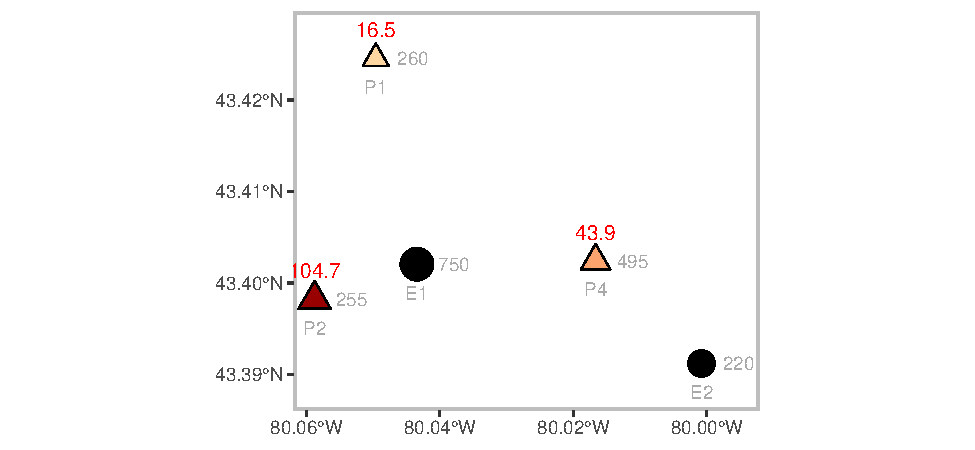
\includegraphics[width=1\linewidth]{Spatial-Availability-Refreshed_files/figure-latex/toy-example-accessibility-plot-1} \caption{\label{fig:toy-example-accessibility}Accessibility to jobs (red text) from population centers (P) to employment centers (E) for the synthetic example. Values of population and employment are shown in white text.}\label{fig:toy-example-accessibility-plot}
\end{figure}

Gavity-based accessibility has been shown to be an excellent indicator
of the intersection between urban structure and transportation
infrastructure (Kwan, 1998; Reggiani et al., 2011; Shi et al., 2020).
However, beyond enabling comparisons of relative values they are not
highly interpretable on their own (Miller, 2018). For instance, from
Figure \ref{fig:toy-example-accessibility}, P1 has lower accessibility
than P2 but despite the accessibility value for P1 being relatively low
it is still better than \emph{zero}. On the other hand, P2 has high
accessibility, but is this accessibility excellent, good, or only fair?
What does it \emph{mean} for a location to have accessibility to so many
jobs?

To address this interpretability issue, previous research has aimed to
index and normalize values on a per demand-population basis (e.g.,
Barboza et al., 2021; Pereira et al., 2019; Wang et al., 2021). However,
as recent research on accessibility discusses (Allen and Farber, 2019;
Kelobonye et al., 2020; Merlin and Hu, 2017; Paez et al., 2019), these
steps do not truly address competition. In effect, when calculating
\(A_i\), every opportunity enters the weighted sum once for every origin
\(i\) that can reach it. Put another way, if a densely populated
population center pops up next to P2 this center too will have a high
accessibility score. There is a lurking assumption in this process that
all opportunities are \emph{available} to anyone from any origin
\(i=1,\cdots,n\) who can reach them: in other words, opportunities are
assumed to be infinitely divisible and thus inexhaustible. This
multiplication of the opportunities means that competition is not really
present, and \(A_i\) does not consider that neighbouring population
centers are seeking the same exhaustible opportunities. Neglecting to
constrain opportunity counts (i.e., single-constraint) in addition to
obscuring the interpretability of accessibility can also bias the
estimated landscape of opportunity, as we will discuss later on in the
paper.

\hypertarget{measures-with-congestion-andor-competition}{%
\subsection{Measures with congestion and/or
competition}\label{measures-with-congestion-andor-competition}}

Past research has considered both congestion and/or competition in
accessibility analysis. The highly cited work of (1998) for example,
divides conventional accessibility by the travel-cost adjusted
population seeking the opportunities in a given region: this was perhaps
the first measure of accessibility to introduce congestion. This work
was popularized by the 2-step floating catchment approach (2SFCA)
introduced by (2003) and widely used today.

A synthetic example of a three population center and two employment
centre is solved using this popular competitive measure and shown in
Table XX- left. The formulation of the 2SFCA approach is shown in step 1
(Equation (\ref{eq:2SFCA-step1})) where the PPR \(R_j\) is calculated
for each opportunity and then allocated to populations based on travel
cost \(f(\cdot)\) in step 2 (Equation (\ref{eq:2SFCA-step2})). The
synthetic example is solved in detail for the 2SFCA and all other
accessibility measures in the Appendix (XX).

\begin{equation}
\label{eq:2SFCA-step1}
R_{j} = \frac{O_{j}}{\sum_i P_{i} \cdot f(c_{ij})}\\
\end{equation}

\begin{equation}
\label{eq:2SFCA-step2}
A_{i} = {\sum_j R_{j} \cdot f(c_{ij})}\\
\end{equation}

\noindent where:

\begin{itemize}
\tightlist
\item
  \(A\) is accessibility.
\item
  \(i\) is a set of origin locations.
\item
  \(j\) is a set of destination locations.
\item
  \(O_j\) is the number of opportunities at location \(j\);
\item
  \(P_i\) is the population at location \(i\); \(\sum_j R_j\) is the
  total supply of opportunities in the study region.
\item
  \(R_j\) is the provider-to-population (PPR) ratio at location \(j\);
\item
  \(c_{ij}\) is a measure of the cost of moving between \(i\) and \(j\);
\item
  \(f(\cdot)\) is an impedance function of \(c_{ij}\).
\end{itemize}

As shown by Paez et al. (2019), congestion does not necessarily mean
competition, as the same population is claimed by multiple service
centers and the same level of service is given to multiple populations.

Other measures have been proposed that include inverse balancing factors
as in (Horner, 2004) and (Allen and Farber, 2019). These methods
involves computing the inverse balancing factor for each origin through
an iterative procedure until convergence. The iterations seek to match
the travel-cost weighted opportunities to the travel-cost weighted
population in the region. It requires that the total population and
opportunities are equal in the region but the mean accessibilities from
previous iterations can be included to standardize the imbalance. The
solved synthetic example is in Table XX - middle, and the formulation of
this method is as follows in Equation (\ref{eq:Inverse-balancing-1}) and
(\ref{eq:Inverse-balancing-2}).

\begin{equation}
\label{eq:Inverse-balancing-1}
A_{i} = \frac{\bar A^{o}}{\bar A^{c}}{\sum_{j=1}^{J} \frac{O_{j}f(c_{ij})}{B_{j}}}\\
\end{equation}

\begin{equation}
\label{eq:Inverse-balancing-2}
B_{i} = {\sum_{i=1}^{I} \frac{P_{i}f(c_{ij})}{A_{i}}}\\
\end{equation}

\noindent where: - \(B_{i}\) is the balancing factor; other variables
defined in the gravity model.

Incorporating the concept of balance between the population and
opportunities, a recent advancement to the 2SFCA is the balanced 2-step
floating catchment approach (B2SFCA) of (Paez et al., 2019). In both
steps, the number of opportunities from the PPR to each origin, this
results in a consistent number of opportunities being assigned.

In the B2SFCA, the PPR \(R_{j}\) for each employment center can be
interpreted as the total number of jobs accessible to the total
population after being \emph{proportionally} adjusted to the travel
cost. The PPR \(R_{j}\) is then allocated, proportionally based on
travel cost, to each employment center. For this reason, the sum of all
\(A_{i}\) adds up to the same value as the sum of all \(R_{j}\). Since
PPR and the subsequent \(A_{i}\) are proportionally allocated based
travel costs, it should be noted that \(A_{i}\) no longer considers
\emph{potential} interaction in the how it was defined in the gravity
model (Hansen, 1959) and instead represent the allocation of PPR, based
on travel time, to each population. This measure introduces some
consistency in how the PPR is calculated (compared to the 2SFCA), but is
still lacking interpretability in the resulting values.

The solved synthetic example is in Table XX - right, and the formulation
of this method is as follows in Equation (\ref{eq:B2SFCA-1}) and
(\ref{eq:B2SFCA-2}).

\begin{equation}
\label{eq:B2SFCA-1}
R_{j} = \frac{O_{j}}{\sum_i P_{i} \frac{f(c_{ij})}{\sum_j f(c_{ij})}}\\
\end{equation}

\begin{equation}
\label{eq:B2SFCA-2}
A_{i} = {\sum_j R_{j}\frac{f(c_{ij})}{\sum_j f(c_{ij})}}\\
\end{equation}

\hypertarget{introducing-spatial-availability}{%
\section{Introducing spatial
availability}\label{introducing-spatial-availability}}

Here we introduce the spatial availability model formulation and
demonstrate how it compares to other measures of accessibility with
congestion and/or competition.

We define spatial availability \(V_{i}\) as the number of opportunities
\(O\) that are proportionally allocated based on population and cost of
travel, for all origins \(i\) to all destinations \(j\).

This idea is reflected in Equation (\ref{eq:spatial-availability}),
where \(F^p_{i}\) is a population-based allocation factor that grants a
larger share of the existing opportunities to larger centers, and
\(F^c_{ij}\) is a transportation cost-based allocation factor that
grants a larger share of the existing opportunities to closer centers.
This is in line with the tradition of gravity modeling, and proposed
framework distinguishes between opportunities at a destination and
demand for opportunities at the origin.

\begin{equation}
\label{eq:spatial-availability}
V_{i} = O_j\frac{F^p_{i} \cdot F^c_{ij}}{\sum_{i=1}^K F^p_{i} \cdot F^c_{ij}}
\end{equation}

The terms in Equation \ref{eq:spatial-availability} are as follows:

\begin{itemize}
\tightlist
\item
  \(V_{i}\) is the spatial availability of opportunities in \(j\) to
  origin \(i\).
\item
  \(i\) is a set of origin locations in the region \(K\).
\item
  \(j\) is a set of destination locations in the region \(K\).
\item
  \(O_j\) is the number of opportunities at location \(j\) in the region
  \(K\).
\item
  \(F^p_{i}\) is a proportional allocation factor of the population in
  \(i\).
\item
  \(F^c_{ij}\) is a proportional allocation factor of travel cost for
  \(i\); it is a product of a monotonically decreasing (i.e., impedance)
  function associated with the cost of travel between \(i\) and \(j\).
\end{itemize}

Notice that, unlike \(A_i\) in Equation
(\ref{eq:conventional-accessibility}), the population in the region
enters the calculation of \(V_{i}\). It is important to detail the role
of the two proportional allocations factors in the formulation of
spatial availability. We begin by considering the population allocation
factor \(F^p_{i}\) followed by the role of the travel cost allocation
factor \(F^c_{ij}\); then we show how both allocation factors combine in
the final general form of spatial availability \(V_{i}\). The
calculation of spatial availability is introduced with a step-by-step
example for synthetic three population centers (\(P_1\), \(P_2\),
\(P_4\)) in the role of demand (i.e., the number of individuals in the
labor market who `demand' employment) and two employment centers
(\(O_1\), \(O_2\)) in the role of opportunities.

\hypertarget{population-and-travel-cost-allocation-factors}{%
\subsection{Population and travel cost allocation
factors}\label{population-and-travel-cost-allocation-factors}}

We begin with allocation based on demand by population; consider an
employment center \(j\) with \(O_j\) jobs. In the general case where
there are \(K\) population centers in the region, we define the
following factor:

\begin{equation}
\label{eq:pop-alloc-factor}
F^p_{i} = \frac{P_{i}^\alpha}{\sum_{i=1}^K P_{i}^\alpha}
\end{equation}

The population allocation factor \(F^p_{i}\) corresponds to the
proportion of the population in origin \(i\) relative to the population
in the region. On the right hand side of the equation, the numerator
\(P_{i}\) is the population at origin \(i\) that is eligible for and
demands jobs \(j\). The summation in the denominator is over
\(i=1,\cdots,K\), the population at origins \(i\) in the region. To
modulate the effect of demand by population in this factor we include an
empirical parameter \(\alpha\) (i.e., \(\alpha <1\) places greater
weight on smaller centers relative to larger ones while \(\alpha>1\)
achieves the opposite effect). This population allocation factor
\(F^p_{i}\) can now be used to proportionally allocate a share of the
jobs at \(j\) to origins.

More broadly, since the factor \(F^p_{i}\) is a proportion, when it is
summed over \(i=1,\cdots,K\) it always equals to 1 (i.e.,
\(\sum_i^{K} F^p_{i} = 1\)). This is notable since the share of jobs at
each destination \(j\) allocated to (i.e., available to) each origin,
based on population, is equal to \(V^p_{i} = O_j \cdot F^p_{i}\). Since
the sum of \(F^p_{i}\) is equal to 1, it follows that
\(\sum_{i=1}^I V_{i} = O_j\). In other words, the number of
opportunities (jobs) across the region is preserved. The result is a
proportional allocation of jobs to origins based on the size of their
populations.

For simplicity, assume that \(\alpha=1\). The population allocation
factors \(F^p_{i}\) is as follows in Equation
(\ref{eq:pop-alloc-factor-2populations}).

\begin{equation}
\label{eq:pop-alloc-factor-2populations}
\begin{array}{l}
F^p_{1} = \frac{P_1 ^\alpha}{P_1^\alpha + P_2^\alpha + P_3^\alpha} = \frac{260}{260 + 255 + 495} = 0.257\\
F^p_{2} = \frac{P_2^\alpha}{P_1^\alpha + P_2^\alpha + P_3^\alpha}  = \frac{255}{260 + 255 + 495} = 0.252\\
F^p_{3} = \frac{P_3^\alpha}{P_1^\alpha + P_2^\alpha + P_3^\alpha}  = \frac{495}{260 + 255 + 495} = 0.490\\
\end{array}
\end{equation}

These \(F^p_{i}\) values can be used to find a \emph{partial} spatial
availability in which jobs are allocated proportionally to population;
this partial spatial availability \(V^p_{i}\) for each population center
is calculated as follows in Equation
(\ref{eq:pop-alloc-factor-SA-2populations}).

\begin{equation}
\label{eq:pop-alloc-factor-SA-2populations}
\begin{array}{l}
V^p_{1} = O_1 \cdot F^p_{1} + O_2 \cdot F^p_{1} = 750 \cdot 0.257 + 220 \cdot 0.257 = 249.29 \\
V^p_{2} = O_1 \cdot F^p_{2} + O_2 \cdot F^p_{2} = 750 \cdot 0.252 + 220 \cdot 0.252 = 244.44 \\
V^p_{3} = O_1 \cdot F^p_{3} + O_2 \cdot F^p_{3}= 750 \cdot 0.490 + 220 \cdot 0.490 = 475.30 \\
\end{array}
\end{equation}

When using only the proportional allocation factor \(F^p_{i}\) to
calculate spatial availability (differentiated here by being defined as
\(V^p_{i}\) instead of \(V_{i}\)), proportionally more jobs are
allocated to the bigger population center (i.e., 2 times more jobs as it
is 2 times larger in population). We can also see that the sum of
spatial availability for all population centers equals the total number
of opportunities.

Clearly, using only the proportional allocation factor \(F^p_{i}\) to
calculate spatial availability does not account for how far population
centers are from employment centers. It is the task of the second
allocation factor \(F^c_{ij}\) to account for the friction of distance,
as seen in Equation (\ref{eq:tcost-alloc-factor}).

\begin{equation}
\label{eq:tcost-alloc-factor}
F^c_{ij} = \frac{f(c_{ij})}{\sum_{i=1}^K f(c_{ij})}\\
\end{equation}

Travel cost allocation factor \(F^c_{ij}\) serves to proportionally
allocate more jobs to closer locations through an impedance function.
\(c_{ij}\) is the cost (e.g., the distance, travel time, etc.) to reach
employment center \(j\) from \(i\) and \(f(\cdot)\) is an impedance
function that depends on cost (\(c_{ij}\)).

To continue with the example, assume that the impedance function is a
exponential function with \(\beta=-0.00015\) and the distance from
population centers to employment centers is as shown in TABLE XX.
\(\beta\) modulates the steepness of the impedance effect and is
empirically determined in the case of positive accessibility, or set by
the analyst to meet a preset condition in the case of normative
accessibility (Paez et al., 2012). The proportional allocation factor
\(F^p_{i}\) for all population centers is defined in Equation
(\ref{eq:tcost-allocation-factor-2populations}).

\begin{equation}
\label{eq:tcost-allocation-factor-2populations}
\begin{array}{l}
F^c_{1,1} = \frac{\exp(\beta*2548.1)}{\exp(\beta *2548.1) + \exp(\beta *1314.1) + \exp(\beta *2170.2)} = 0.109\\
F^c_{2,1} = \frac{\exp(\beta *1314.1)}{\exp(\beta *2548.1) + \exp(\beta *1314.1) + \exp(\beta *2170.2)} = 0.697\\
F^c_{3,1} = \frac{\exp(\beta *2170.2)}{\exp(\beta *2548.1) + \exp(\beta *1314.1) + \exp(\beta *2170.2)} = 0.193\\
F^c_{1,2} = \frac{\exp(\beta*5419.1)}{\exp(\beta *5419.1) + \exp(\beta *2170.2) + \exp(\beta *1790.1)} = 0.004\\
F^c_{2,2} = \frac{\exp(\beta *4762.6)}{\exp(\beta *5419.1) + \exp(\beta *2170.2) + \exp(\beta *1790.1)} = 0.011\\
F^c_{3,2} = \frac{\exp(\beta *1790.1)}{\exp(\beta *5419.1) + \exp(\beta *2170.2) + \exp(\beta *1790.1)} = 0.984\\
\end{array}
\end{equation}

We can see, for instance, that the proportional allocation factor for
\(P_2\) is largest for \(E_1\) since the cost (i.e., distance) to
\(E_1\) is lowest. For \(E_2\), \(P_3\) has the largest proportional
allocation factor similarly because it is in the closest proximity.
Using the travel cost proportional allocation factors \(F^c_{ij}\) as
defined in Equation (\ref{eq:tcost-allocation-factor-2populations}), we
can calculate the spatial availability of jobs for each population
center based only on \(F^c_{ij}\) and the jobs available at each
employment center, as shown in Equation
(\ref{eq:tcost-allocation-factor-SA-2populations}).

\begin{equation}
\label{eq:tcost-allocation-factor-SA-2populations}
\begin{array}{l}
V^c_{1,1} = E_1 \cdot F^c_{1,1} = 750 \times 0.109 = 81.75\\
V^c_{2,1} = E_1 \cdot F^c_{2,1} = 750 \times  0.697 = 522.75\\
V^c_{3,1} = E_1 \cdot F^c_{3,1} = 750 \times  0.193 = 144.75\\
V^c_{1,2} = E_2 \cdot F^c_{1,2} = 220 \times 0.004 = 0.88\\
V^c_{2,2} = E_2 \cdot F^c_{2,2} = 220 \times  0.011 = 2.42\\
V^c_{3,2} = E_2 \cdot F^c_{3,2} = 220 \times  0.984 = 216.48\\
\end{array}
\end{equation}

For instance, spatial availability defined by \(F^c_{ij}\) only (i.e.,
\(V^c_{i}\)) allocates a largest share of jobs from \(E_1\) to \(P_2\)
since it is the closest. However, as previously discussed, \(P_2\) has a
relatively small population, so \(V^p_{2,1}\) is actually the smallest
value of any population center for \(E_1\). It is necessary to combine
both population and travel cost factors to better reflect demand; these
two components are in line with how demand is conventionally modelled in
accessibility calculations which are re-scaled on a per
demand-population basis or also consider competition (e.g., Allen and
Farber, 2019; Barboza et al., 2021; Yang et al., 2006). Fortunately,
since both \(F^c_{ij}\) and \(F^p_{i}\) preserve the total number of
opportunities as they independently sum to 1, they can be combined
multiplicatively to calculate the proposed spatial availability
\(V_{i}\) which considers demand to be based on both population and
travel cost.

\hypertarget{putting-spatial-availability-together}{%
\subsection{Putting spatial availability
together}\label{putting-spatial-availability-together}}

We can combine the proportional allocation factors by population
\(F^p_{i}\) and travel cost \(F^c_{ij}\) and calculate spatial
availability \(V_{i}\) as introduced in Equation
(\ref{eq:spatial-availability}) and repeated below:

\[
V_{i} = O_j\frac{F^p_{i} \cdot F^c_{ij}}{\sum_{i=1}^K F^p_{i} \cdot F^c_{ij}}
\]

The resulting spatial availability \(V_{i}\) is calculated for all
population centers is calculated in Equation (\ref{eq:SA-2populations}).

\begin{equation}
\label{eq:SA-2populations}
\begin{array}{l}

V_{1,1} = O_1\cdot \frac{F^p_{1,1} \cdot F^c_{1,1}}{F^p_{1,1} \cdot F^c_{1,1} + F^p_{2,1} \cdot F^c_{2,1} + F^p_{3,1} \cdot F^c_{3,1}} = 
750 \cdot \frac{0.26 \cdot 0.109}{0.26 \cdot 0.109 + 0.25 \cdot 0.697 + 0.49 \cdot 0.193} = 70.45\\
V_{2,1} = O_1\cdot \frac{F^p_{2,1} \cdot F^c_{2,1}}{F^p_{1,1} \cdot F^c_{1,1} + F^p_{2,1} \cdot F^c_{2,1} + F^p_{3,1} \cdot F^c_{3,1}} = 
750 \cdot \frac{0.25 \cdot 0.697}{0.26 \cdot 0.109 + 0.25 \cdot 0.697 + 0.49 \cdot 0.193} = 441.72\\
V_{3,1} = O_1\cdot \frac{F^p_{3,1} \cdot F^c_{3,1}}{F^p_{1,1} \cdot F^c_{1,1} + F^p_{2,1} \cdot F^c_{2,1} + F^p_{3,1} \cdot F^c_{3,1}} = 
750 \cdot \frac{0.49 \cdot 0.193}{0.26 \cdot 0.109 + 0.25 \cdot 0.697 + 0.49 \cdot 0.193} = 237.83\\

V_{1,2} = O_2\cdot \frac{F^p_{1,2} \cdot F^c_{1,2}}{F^p_{1,2} \cdot F^c_{1,2} + F^p_{2,2} \cdot F^c_{2,2} + F^p_{3,2} \cdot F^c_{3,2}} = 
220 \cdot \frac{0.26 \cdot 0.004}{0.26 \cdot 0.004 + 0.25 \cdot 0.011 + 0.49 \cdot 0.984} = 0.46\\
V_{2,2} = O_2\cdot \frac{F^p_{2,2} \cdot F^c_{2,2}}{F^p_{1,2} \cdot F^c_{1,2} + F^p_{2,2} \cdot F^c_{2,2} + F^p_{3,2} \cdot F^c_{3,2}} = 
220 \cdot \frac{0.25 \cdot 0.011}{0.26 \cdot 0.004 + 0.25 \cdot 0.011 + 0.49 \cdot 0.984} = 1.26\\
V_{3,2} = O_2\cdot \frac{F^p_{1,2} \cdot F^c_{1,2}}{F^p_{1,2} \cdot F^c_{1,2} + F^p_{2,2} \cdot F^c_{2,2} + F^p_{3,2} \cdot F^c_{3,2}} = 
220 \cdot \frac{0.49 \cdot 0.984}{0.26 \cdot 0.004 + 0.25 \cdot 0.011 + 0.49 \cdot 0.984} = 218.28\\
\end{array}
\end{equation}

Aggregating by population center gives the following values:

\begin{equation}
\label{eq:SA-2populations-2}
\begin{array}{l}
V_{1} = 70.45 + 0.46 = 70.91\\
V_{2} = 441.72 + 1.26 = 442.98\\
V_{3} = 237.83 + 218.28 = 456.11\\
\end{array}
\end{equation}

Considering both population and cost allocation factors in \(V_{i}\),
the jobs at \(E1\) that are allocated to all population centers are
still preserved (i.e., \(V_{1,1} + V_{2,1} + V_{3,1} = O_1\)).
Additionally, the sum of jobs at \(E2\) are also all preserved (i.e.,
\(V_{1,2} + V_{2,2} + V_{3,2} = O_2\)). Thus the sum of \(V_{i}\) equals
the sum of opportunities (i.e., ) Notice that \(V_{i}\), allocates a
number of jobs to \(P_1\), \(P_2\), and \(P_3\) is between the values
allocated in \(V^p_{i}\) and \(V^c_{i}\).

When comparing \(V_i\) to the singly-constrained gravity model (see
Wilson (1971)), \(V_i\) is the result of constraining \(A_i\) to match
one of the marginals in the origin-destination table, the known total of
opportunities. Since the sum of opportunities is preserved in the
procedures above, it is possible to calculate an interpretable measure
of spatial availability per capita (lower-case \(v_i\)) as shown in
Equation (\ref{eq:SA-per-capita}).

\begin{equation}
\label{eq:SA-per-capita}
v_i = \frac{V_i}{P_i}
\end{equation}

To complete the illustrative example, the per capita spatial
availability of jobs is calculated in Equation
(\ref{eq:SA-per-capita-2populations}).

\begin{equation}
\label{eq:SA-per-capita-2populations}
\begin{array}{l}
v_{1} = \frac{V_{1,1} + V_{1,2}}{P_1} =  \frac{70.91}{260} = 0.272\\
v_{2} =  \frac{V_{2,1} + V_{2,2}}{P_2} =  \frac{442.98}{255} = 1.737\\
v_{3} =  \frac{V_{3,1} + V_{3,2}}{P_3} =  \frac{456.11}{495} = 0.921\\
\end{array}
\end{equation}

We can see that since \(P_2\) is closest to \(E1\), is similarly spaced
out from \(P1\) and \(P2\), and is a smaller population center thus
having less competition, \(P_2\) benefits with a higher spatial
availability of jobs per job-seeking population. We can also compare
these values to the overall ratio of jobs-to-population in this region
of two job center and three population centers is
\(\frac{750+220}{260+255+495}=\) 0.96 jobs per person.

\begin{table}

\caption{\label{tab:all-access-measures-examples-table}\label{tab:all-access-measures-examples-table}Summary of reviewed accessibility methods calculated for the synthetic example}
\centering
\begin{tabular}[t]{llll}
\toprule
  & P1 & P2 & P3\\
\midrule
Conv. Gravity & 16.5 & 104.65 & 43.93\\
2SFCA & 0.27 & 1.74 & 0.92\\
B2SFCA & 0.12 & 0.77 & 0.88\\
Inverse Balancing & 14.56 & 92.35 & 47.05\\
V\_i & 70.91 & 442.98 & 456.11\\
\addlinespace
v\_i & 0.27 & 1.74 & 0.92\\
\bottomrule
\end{tabular}
\end{table}

\hypertarget{empirical-example-of-toronto}{%
\section{Empirical example of
Toronto}\label{empirical-example-of-toronto}}

In this section we use population and employment data from the Golden
Horseshoe Area (GGH). This is the largest metropolitan region in Canada
and includes the cities of Toronto and Hamilton. We calculate gravity
accessibility, XXX, and the proposed spatial availability for Toronto
after introducing the data used and calibrating an impedance function.

\hypertarget{data}{%
\subsection{Data}\label{data}}

Population and employment data are drawn from the 2016 Transportation
Tomorrow Survey (TTS). This survey collects representative urban travel
information from 20 municipalities contained within the GGH area in the
southern part of Ontario, Canada (see Figure
\ref{fig:TTS-16-survey-area}) (Data Management Group, 2018). The data
set includes Traffic Analysis Zones (TAZ) (n=3,764), the number of jobs
(n=3,081,885) and workers (n=3,446,957) at each origin and destination.
The TTS data is based on a representative sample of between 3\% to 5\%
of households in the GGH and is weighted to reflect the population
covering the study area has a whole (Data Management Group, 2018).

To generate the travel cost for these trips, travel times between
origins and destinations are calculated for car travel using the R
package \{r5r\} (Rafael H. M. Pereira et al., 2021) with a street
network retrieved from OpenStreetMap for the GGH area. A the 3 hr travel
time threshold was selected as it captures 99\% of population-employment
pairs (see the travel times summarized in Figure
\ref{fig:TTS-16-survey-area}). This method does not account for traffic
congestion or modal split, which can be estimated through other means
(e.g., Allen and Farber, 2021; Higgins et al., 2021). For simplicity, we
carry on with the assumption that all trips are taken by car in
uncongested travel conditions.

All data and data preparation steps are documented and can be freely
explored in the companion open data product
\href{https://github.com/soukhova/TTS2016R}{\{TTS2016R\}}.

\begin{figure}

{\centering 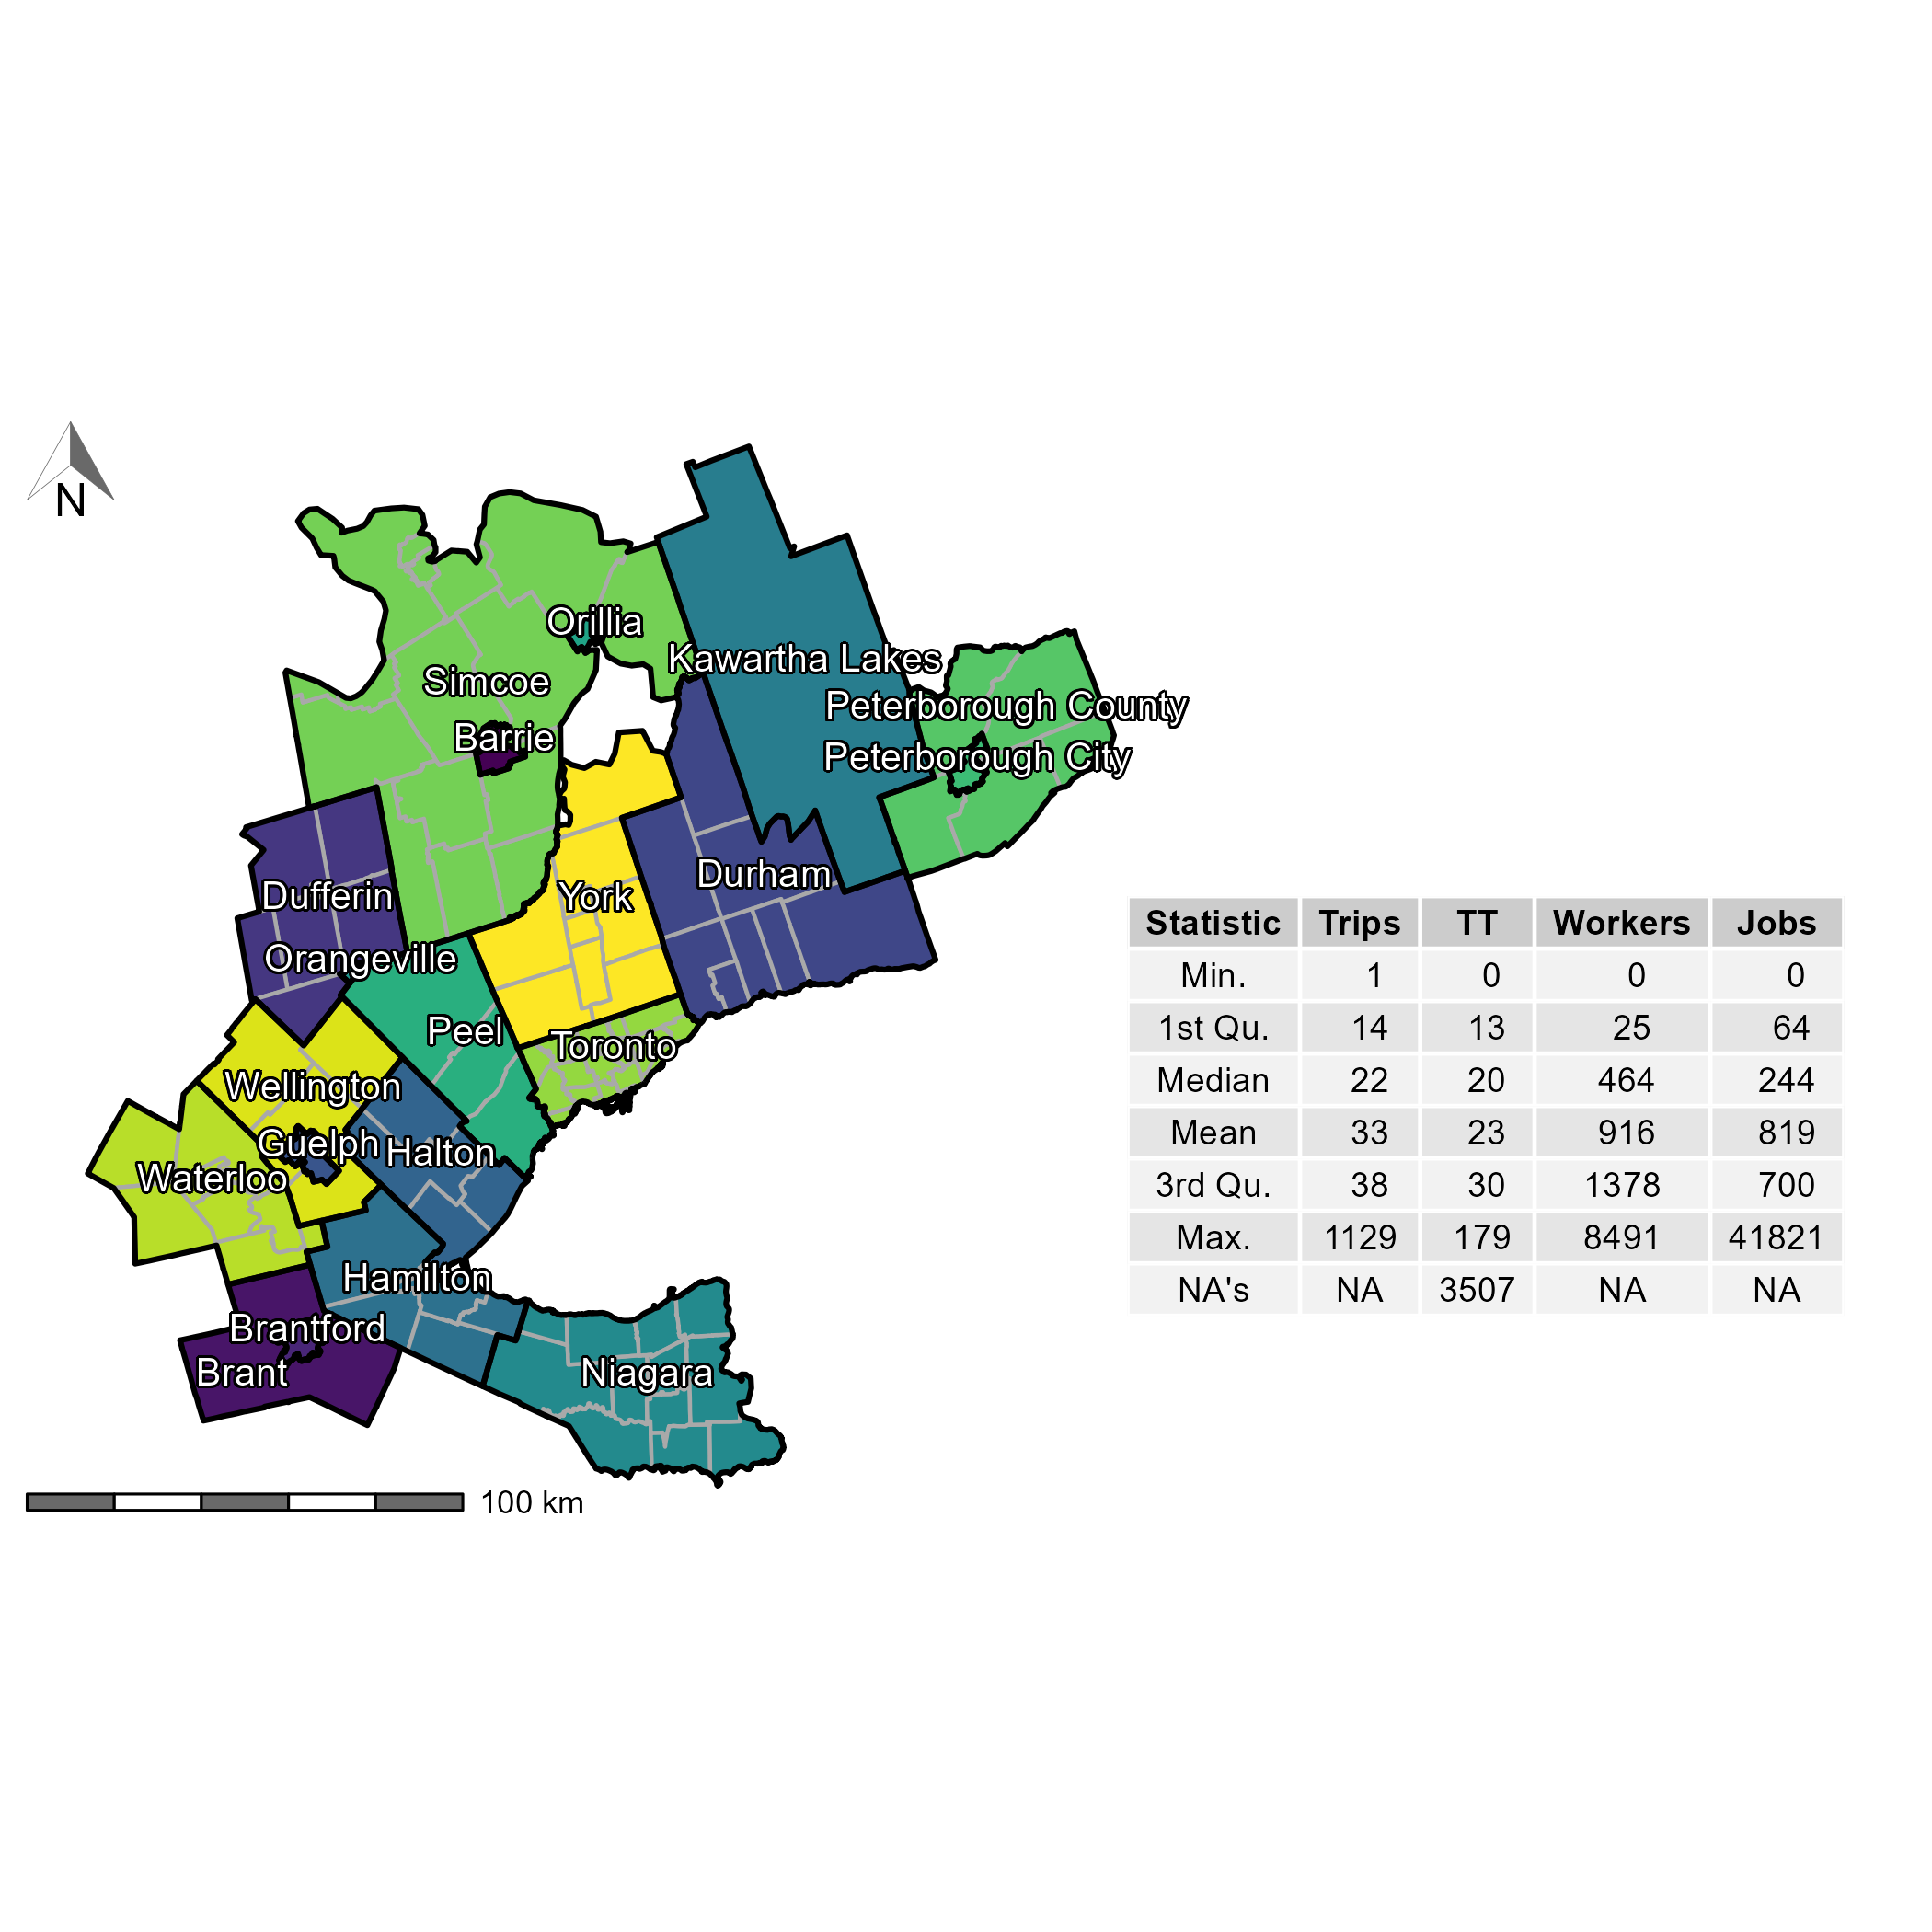
\includegraphics[width=0.8\linewidth]{images/TTS16-survey-area} 

}

\caption{\label{fig:TTS-16-survey-area}TTS 2016 study area (GGH, Ontario, Canada) along with the descriptive statistics of the trips, calculated origin-destination car travel time (TT), workers per TAZ, and jobs per TAZ. Contains 20 regions (black boundaries) and sub-regions (dark gray boundaries).}\label{fig:TTS-16-survey-area}
\end{figure}

\hypertarget{calibration-of-an-impedance-function}{%
\subsection{Calibration of an impedance
function}\label{calibration-of-an-impedance-function}}

In the synthetic example introduced in a preceding section, a negative
exponential function with an arbitrary parameter was used. For the
empirical example, we calibrate an impedance function on the trip length
distribution (TLD) of commute trips. Briefly, a TLD represents the
proportion of trips that are taken at a specific travel cost (e.g.,
travel time); this distribution is commonly used to derive impedance
functions in accessibility research (Batista et al., 2019; Horbachov and
Svichynskyi, 2018).

The empirical and theoretical TLD for this data set are represented in
the top-left panel of Figure \ref{fig:TLD-Gamma-plot}. Maximum
likelihood estimation and the Nelder-Mead method for direct optimization
available within the \{fitdistrplus\} package (Delignette-Muller and
Dutang, 2015) were used. Based on goodness-of-fit criteria and
diagnostics seen in Figure \ref{fig:TLD-Gamma-plot}, the gamma
distribution was selected (also see Figure \ref{fig:plot-cullen-frey} in
Appendix XX).

\begin{verbatim}
[1] 3069541
\end{verbatim}

\begin{figure}

{\centering 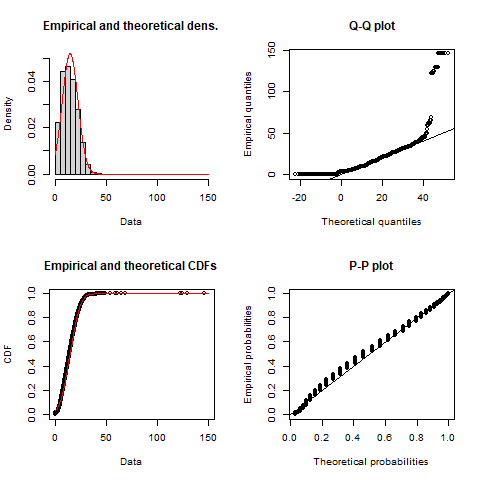
\includegraphics[width=0.8\linewidth]{images/impedance_function} 

}

\caption{\label{fig:TLD-Gamma-plot}Car trip length distribution and calibrated gamma distribution impedance function (red line) with associated Q-Q and P-P plots. Based on TTS 2016.}\label{fig:TLD-Gamma-plot}
\end{figure}

The gamma distribution takes the following general form where the
estimated `shape' is \(\alpha=\) 2.019, the estimated `rate' is
\(\beta =\) 0.094, and \(\Gamma(\alpha)\) is defined in Equation
(\ref{gamma-dist}).

\begin{equation}
\label{gamma-dist}
\begin{array}{l} 
f(x, \alpha, \beta) = \frac {x^{\alpha-1}e^{-\frac{x}{\beta}}}{ \beta^{\alpha}\Gamma(\alpha)} \quad \text{for } 0 \leq x \leq \infty\\

\Gamma(\alpha) =  \int_{0}^{\infty} x^{\alpha-1}e^{-x} \,dx\\
\end{array}
\end{equation}

\hypertarget{measuring-access-to-jobs-in-toronto}{%
\subsection{Measuring access to jobs in
Toronto}\label{measuring-access-to-jobs-in-toronto}}

Toronto is the largest city in the GGH and represents a significant
subset of workers and jobs in the GGH; 31\% of workers in the GGH travel
to jobs in Toronto and 40\% of jobs are located within Toronto.

\begin{figure}
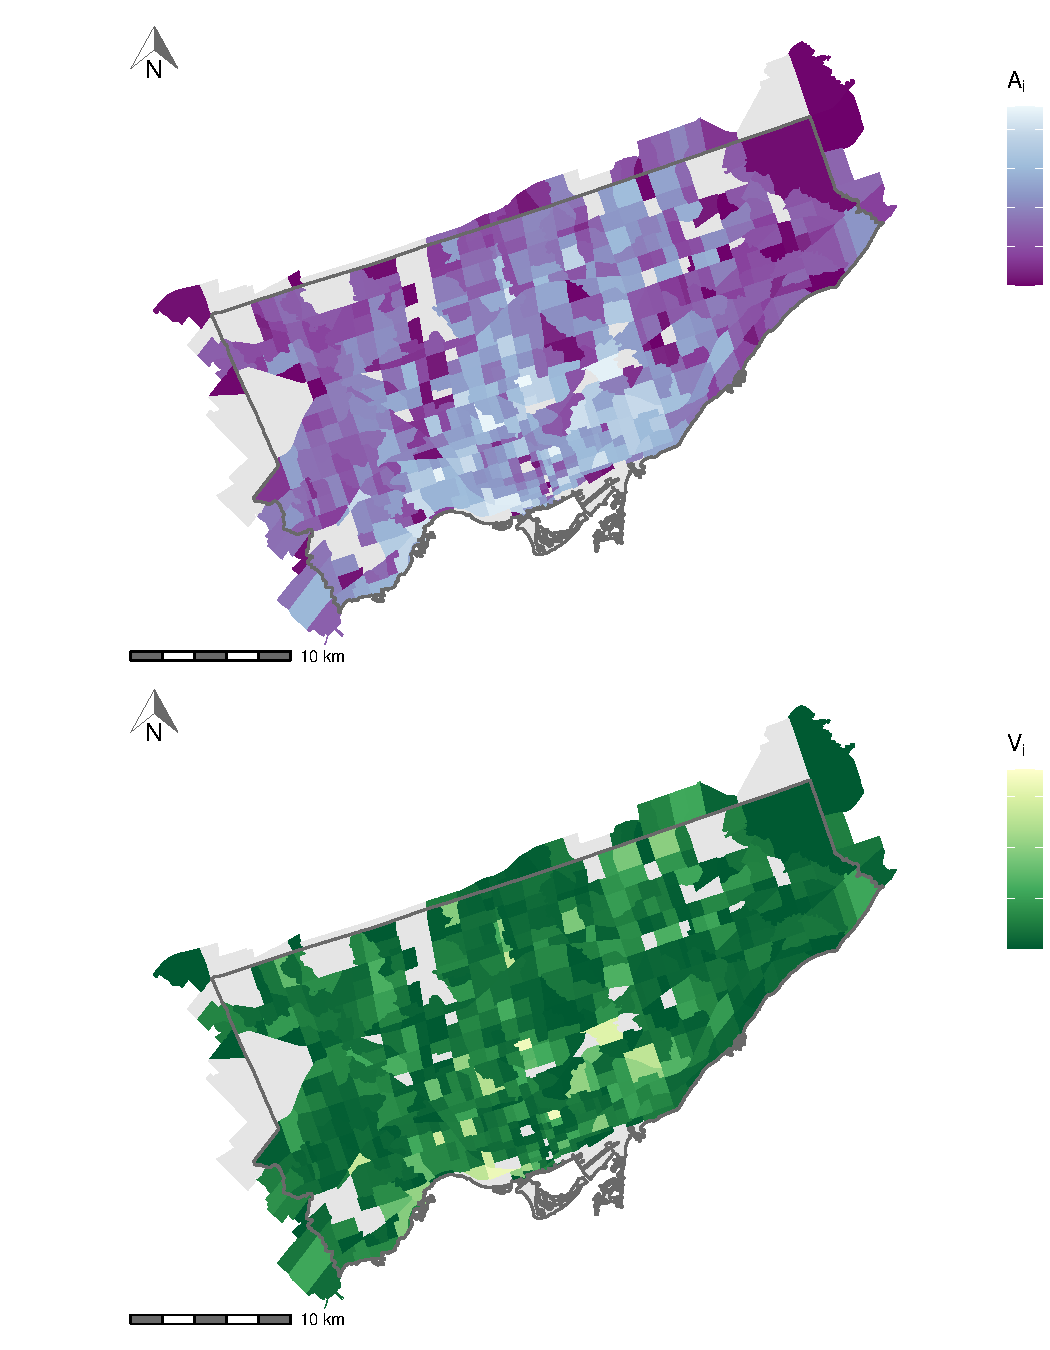
\includegraphics[width=1\linewidth]{Spatial-Availability-Refreshed_files/figure-latex/plot-access-SA-TO-1} \caption{\label{fig:plot-access-SA-TO}Calculated accessibility (top) and spatial availability (bottom) of employment from origins in destinations and origins in Toronto. Greyed out TAZ represent null accessibility and spatial availability values.}\label{fig:plot-access-SA-TO}
\end{figure}

To enhance the interpretability, spatial availability can be normalized
to provide more meaningful insight into how many jobs are
\emph{available} on average for each TAZ. This normalization, shown in
Figure \ref{fig:plot-avail-GGH-TTS-per-worker}, demonstrates which TAZ
have above (reds) and below (blue) the average available jobs per worker
in the GGH (1.17). Similar to the spatial availability plot of the GGH
jobs in Figure \ref{fig:plot-access-SA-GGH-TTS}, we can see that many
average or above average jobs per worker TAZ (whites and reds) are
present in southern Peel and Halton (south-west of Toronto), Waterloo
and Brantford (even more south-west of Toronto), and Hamilton and
Niagara (south of Toronto), however, the distribution is uneven and many
TAZ within these areas do have below average values (blues).

Interestingly, when considering \emph{competitive} job access, many
areas outside of Toronto have similar jobs per worker values as TAZ in
Toronto. This is contrary to the notion that since Toronto has high job
access it has a significant density of employment opportunities in the
GGH. Not all jobs in Toronto are \emph{available} since Toronto has a
high density of \emph{competition} in addition to density of jobs
opportunities. For instance, urban centers outside of Toronto such as
those found in Brantford, Guelph, southern Peel, Halton, and Niagara
have TAZ which are far above the the TTS average jobs per worker and
higher than TAZ within Toronto. High job access is not seen in the
accessibility plot which suggests that these less densely populated
urban centers may have sufficient employment opportunities for their
populations; this finding is obscured when only considering the
accessibility measure for job access as will be later discussed.

It is also worth noting that there is almost two times more jobs per
worker in the GGH jobs spatial availability results than the GGH Toronto
spatial availability results. This suggests that all GGH people who work
in the city of Toronto, on average, face more competition for jobs than
all GGH people who work anywhere in the GGH .

\begin{figure}
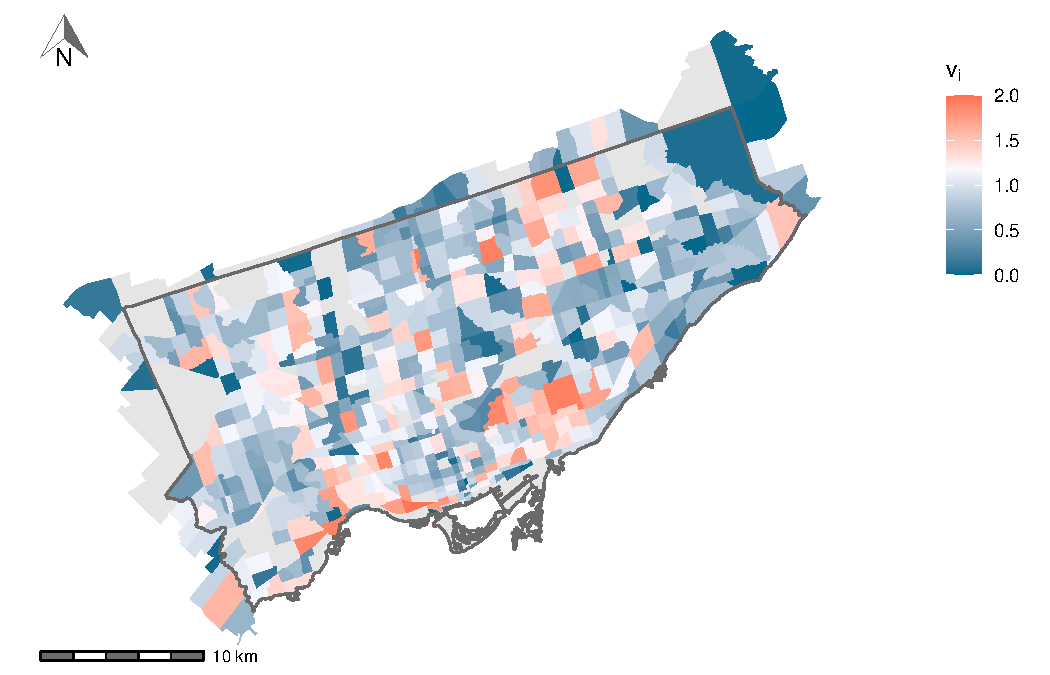
\includegraphics[width=1\linewidth]{Spatial-Availability-Refreshed_files/figure-latex/plot-avail-TO-per-worker-1} \caption{\label{fig:plot-avail-TO-per-worker}Spatial availability per worker, from origins to job opportunities in Toronto.}\label{fig:plot-avail-TO-per-worker}
\end{figure}

\newpage

\hypertarget{discussion-and-conclusions}{%
\section{Discussion and Conclusions}\label{discussion-and-conclusions}}

\hypertarget{appendix-a-step-by-step-accessibility-calculations-for-synthetic-example}{%
\section{Appendix A: Step-by-step accessibility calculations for
synthetic
example}\label{appendix-a-step-by-step-accessibility-calculations-for-synthetic-example}}

Details for the synthetic example:

\begin{table}

\caption{\label{tab:toy-example-table-appendix}\label{tab:toy-example}Summary description of synthetic example}
\centering
\begin{tabular}[t]{llrrr>{}l}
\toprule
Origin & Destination & Population & Jobs & Distance &  \\
\midrule
Population 1 & Employment Center 1 & 260 & 750 & 2548.1 & \\

Population 1 & Employment Center 2 & 260 & 220 & 5419.1 & \\

Population 2 & Employment Center 1 & 255 & 750 & 1314.1 & \\

Population 2 & Employment Center 2 & 255 & 220 & 4762.6 & \\

Population 4 & Employment Center 1 & 495 & 750 & 2170.2 & \\

Population 4 & Employment Center 2 & 495 & 220 & 1790.1 & \multirow{-6}{*}{\raggedright\arraybackslash 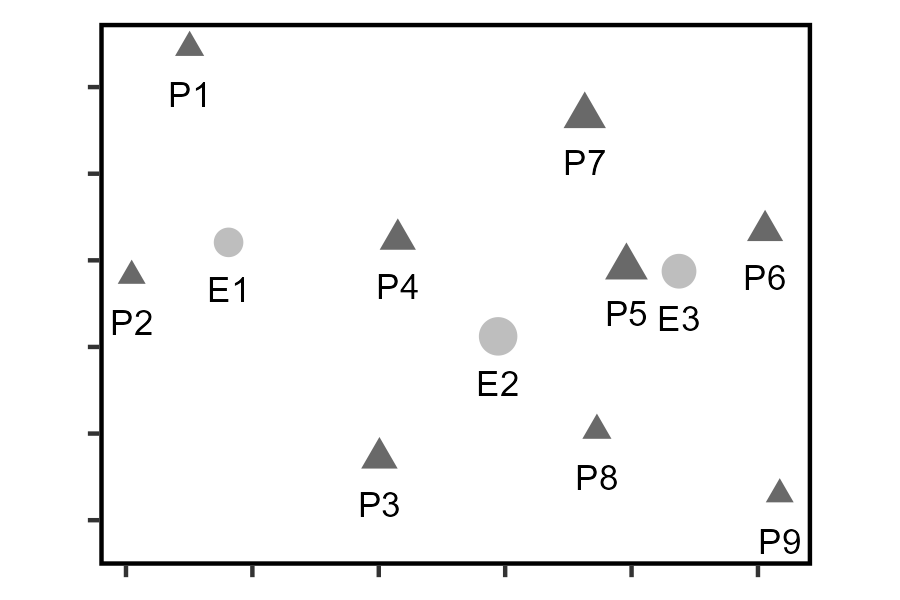
\includegraphics{images/figure-1.png}}\\
\bottomrule
\end{tabular}
\end{table}

\noindent and: \[
\beta = 0.0015 \space in \space f(c_{ij}) = exp(\beta *distance_{ij})
\]

\hypertarget{conventional-gravity-accessibiliy}{%
\subsection{Conventional gravity
accessibiliy}\label{conventional-gravity-accessibiliy}}

\[
A_i = \sum_{j=1}^JO_j \cdot f(c_{ij})
\]

Solved in one step: \[
\sum_{j=1}^JO_j = E1 + E2 =  750 + 220 = 970 \space jobs
\]

\begin{equation}
\begin{array}{l}
A_{P1} = 750 \cdot \exp(-0.0015 *2548.1) + 220 \cdot \exp(-0.0015 *5419.1) = 16.5 \\
A_{P2} = 750 \cdot \exp(-0.0015 *1314.1) + 220 \cdot \exp(-0.0015 *4762.6) = 104.7 \\
A_{P4} = 750 \cdot \exp(-0.0015 *2170.2) + 220 \cdot \exp(-0.0015 *1790.1) = 43.9
\end{array}
\end{equation}

\(A_{P1}\), \(A_{P2}\), and \(A_{P3}\) values represent the number of
travel-cost adjusted opportunities accessible to each population.
Specifically, only a proportion of opportunities are allocated to
population centers based on their travel cost value (higher the travel
cost lower the number of opportunities). The population is not
considered in this measure and the allocation of opportunities is not
constrained, it is only adjusted based on the weight of the travel cost.
With our negative exponential distance decay, accessibility can be as
high as 970 (the total number of opportunities in the region) and as low
as essentially 0.

However, in many instances being close to opportunities doesn't
necessarily mean much practically to an individual nor can this scale of
0 to the maximum number of total opportunities in the region be
operationalized by decision-makers. However, correlates have been found
(XX) so it is a strong indicator of urban structure, but practically
what does it mean for an individual to live in a population center of
\(A_{P4} =\) 43.9 jobs? On a scale of 0 to 970 (\(f(c_{ij})=0\) to
\(f(c_{ij})=1\)), this value is low but of the three population centers
it is around average. However, \(A_{P4}\) also has the largest
population of all population centers. It has a population that is less
than two times the population center of \(A_{P1}\) but an accessibility
value that is greater than two times \(A_{P1}\)'s accessibility value.
Does this mean that accessibility, after adjusting for population, is
greater than in \(P4\)? It is hard to say since the populations have
different travel costs to the opportunities. From this perspective,
competitive measures such as the FCA were introduced with the most
recently popularized 2SFCA (XX) discussed as follows.

\hypertarget{step-floating-catchment-approach-2sfca}{%
\subsection{2 step floating catchment approach
(2SFCA)}\label{step-floating-catchment-approach-2sfca}}

Step one:

\begin{equation}
\begin{array}{l}
R_{j} = \frac{O_{j}}{\sum_i P_{i} \cdot f(c_{ij})}\\

R_{E1} = \frac{750}{260 \cdot \exp(-0.0015 *2548.1) + 255 \cdot \exp(-0.0015 *1314.1) + 495 \cdot \exp(-0.0015 *2170.2)}\\
R_{E1} = 12.4 \space jobs \space per \space travel \space cost \space adjust. \space pop\\
R_{E2} = \frac{220}{260 \cdot \exp(-0.0015 *5419.1) + 255 \cdot \exp(-0.0015 *4762.6) + 495 \cdot \exp(-0.0015 *1790.1)}\\
R_{E2} = 6.5 \space jobs \space per \space travel \space cost \space adjust. \space pop\\
\end{array}
\end{equation}

Step two:

\begin{equation}
\begin{array}{l}
A_{i} = {\sum_j R_{j} \cdot f(c_{ij})}\\
A_{P1} = 12.4 \cdot \exp(-0.0015 *2548.1) + 6.46 \cdot \exp(-0.0015 *5419.1) = 0.27 \\
A_{P2} = 12.4 \cdot \exp(-0.0015 *1314.1) + 6.46 \cdot \exp(-0.0015 *4762.6) = 1.73 \\
A_{P4} = 12.4 \cdot \exp(-0.0015 *2170.2) + 6.46 \cdot \exp(-0.0015 *1790.1) = 0.92
\end{array}
\end{equation}

We see that the PPR \(R_{j}\) for each employment center can be
interpreted as the total number of jobs accessible to the total
travel-cost adjusted population. This step recognizes that not all
opportunities can be distributed to the entire population evenly since
not \emph{all} opportunities can be reached by \emph{all} population
centers. It is assumed that all population and employment centers are in
the same catchment. In step two, \(A_{i}\) values represent the
travel-cost adjusted PPR for each population center. Put another way,
here \(A_{P1}\), \(A_{P2}\), and \(A_{P3}\) values represent the number
of jobs accessible to each population center after being travel-cost
adjusted from both the opportunities-perspective and
population-perspective. The value could theoretically be on a scale of 0
to the maximum total number of PPR in the catchment (i.e.,
\(f(c_{ij})=0\) to \(f(c_{ij})=1\)); in this case that value is 18.9.

The method assumes unconstrained allocation based on travel cost thus
results can be interpreted in a similar way as the conventional gravity
based accessibility but from the perspective of PPR instead of
opportunities. This means that PPR is allocated based on the
\emph{potential} for interaction.

Looking at \(P4\), the largest and most central (to both employment
centers) population center, it has a 3.4 times greater 2SFCA value
compared to \(P1\) (conventional accessibility is only 2.6 times
greater). \(P4\) also has an 2SFCA value which is closer in the value to
\(P2\), it is only 0.53 times smaller than \(P2\) (conventional
accessibility is 0.42 times smaller). Since the 2SFCA adjusts
accessibility from both population-side and opportunity-side
travel-costs, small populations which are close to big employment
centers (\(P2\) close to \(E1\)) but also are in competition with
relatively close and large population centers (\(P4\)) have less
relative accessibility (\(P2\) vs.~\(P4\)) than conventional
accessibility. However, as discussed by Paez et al. (2019), the PPR
calculation in the first step and allocation of PPR to origins in the
second step is not \emph{proportional} to the total population seeking
opportunities. Though the `potential' for interaction is being
consistently allocated in these two steps, when looking to interpret the
measure from the perspective of allocation, the resulting values are
difficult to interpret. This issue of interpretability has been
attempted to be remedied by adjusting the population and opportunities
in both steps by a \emph{proportional} travel cost in the B2SFCA as
follows.

\hypertarget{balanced-2-step-floating-catchment-approach-b2sfca}{%
\subsection{balanced 2 step floating catchment approach
(B2SFCA)}\label{balanced-2-step-floating-catchment-approach-b2sfca}}

Step one:

\begin{equation}
\begin{array}{l}

R_{j} = \frac{O_{j}}{\sum_i P_{i} \frac{f(c_{ij})}{\sum_j f(c_{ij})}}\\

R_{E1} = \frac{750}{260 \frac{\exp(\beta *2548.1)}{\exp(\beta *2548.1) + \exp(\beta *5419.1)} + 255 \frac{\exp(\beta *1314.1)}{\exp(\beta *1314.1) + \exp(\beta *4762.6)} + 495 \frac{\exp(\beta *2170.2)}{\exp(\beta *2170.2) + \exp(\beta *1790.1)}}\\
R_{E2} = \frac{220}{260 \frac{\exp(\beta*5419.1)}{\exp(\beta *2548.1) + \exp(\beta *5419.1)} + 255 \frac{\exp(\beta*4762.6)}{\exp(\beta*1314.1) + \exp(\beta *4762.6)} + 495\frac{\exp(\beta*1790.1)}{\exp(\beta *2170.2) + \exp(\beta *1790.1)}}\\

R_{E1} = 1.09 \space jobs \space per \space proportional \space travel \space cost \space adjust. \space pop\\
R_{E2} = 0.68 \space jobs \space per \space proportional \space travel \space cost \space adjust. \space pop\\
\end{array}
\end{equation}

Step two:

\begin{equation}
\begin{array}{l}
A_{i} = {\sum_j R_{j}\frac{f(c_{ij})}{\sum_j f(c_{ij})}}\\A_{P1} = 1.09\frac{\exp(\beta*2548.1)}{\exp(\beta *2548.1) + \exp(\beta *1314.1) + \exp(\beta *2170.2)} + 0.68 \frac{\exp(\beta*5419.1)}{\exp(\beta *5419.1) + \exp(\beta *2170.2) + \exp(\beta *1790.1)} \\
A_{P2} = 1.09\frac{\exp(\beta *1314.1)}{\exp(\beta *2548.1) + \exp(\beta *1314.1) + \exp(\beta *2170.2)} + 0.68 \frac{\exp(\beta *4762.6)}{\exp(\beta *5419.1) + \exp(\beta *2170.2) + \exp(\beta *1790.1)} \\
A_{P4} = 1.09 \frac{\exp(\beta *2170.2)}{\exp(\beta *2548.1) + \exp(\beta *1314.1) + \exp(\beta *2170.2)} + 0.68 \frac{\exp(\beta *1790.1)}{\exp(\beta *5419.1) + \exp(\beta *2170.2) + \exp(\beta *1790.1)} \\
A_{P1} = 0.12 \\
A_{P2} = 0.77 \\
A_{P4} = 0.88 \\
\end{array}
\end{equation}

In the B2SFCA, the PPR \(R_{j}\) for each employment center can be
interpreted as the total number of jobs accessible to the total
population after being \emph{proportionally} adjusted to the travel
cost. The PPR \(R_{j}\) is then allocated, proportionally based on
travel cost, to each employment center. For this reason, the sum of all
\(A_{i}\) adds up to 1.77, the same value as the sum of all \(R_{j}\).

It should be also noted that when using the \emph{proportional} travel
costs to adjust opportunities and population, instead of using the raw
travel costs as in the 2SFCA, the resulting \(A_{i}\) values are
different. For instance, \(A_{P2}\) is the highest value (1.88 times her
than P4) in the 2SFCA but in the B2SFCA \(A_{P4}\) has the highest
value. In both 2SFCA and conventional accessibility, \(A_{P2}\) is the
highest value since P2 is the most populous population center and has
the closest proximity (low travel cost) to the most populous E1. Though
population size is considered in the first step of 2SFCA, the low
population size of P2 is not significant enough to result in a large
enough decrease in \(A_{P2}\) relative to \(A_{P4}\) (compared to
conventional accessibility in which the acccesibility values between P2
and P4 are relatively greater). However, in B2SFCA, the smaller
population size of P2 has a dramatic impact on the \(A_{P2}\) value.
This is because the travel-cost adjustment is proportional so the
proportionally large population size of P4 results in a smaller PPR for
both employment centers and thus a smaller amount of PPR from E1 is
allocated to P2 in step 2. Since PPR and the subsequent \(A_{i}\) are
proportionally allocated based travel costs, values no longer consider
\emph{potential} interaction and instead represent the allocation of
employment center PPR, based on travel time, to each population center.

This measure introduces some consistency in how the PPR is calculated
and is allocated to P1, P2, and P4, but is still lacking
interpretability in the resulting values.

\hypertarget{inverse-balancing-accessibility-doubly-constrained}{%
\subsection{Inverse Balancing accessibility,
doubly-constrained}\label{inverse-balancing-accessibility-doubly-constrained}}

This measure results in a opportunities per person metric, however, it
constraints opportunities and population from both sides, estimating
accessibility iteratively. The formulation requires the number of
opportunities equals the population so they propose the iterative
estimates are standardized such that opportunities equals population and
the disbalanced is carried through as a factor. The formulation for the
synthetic example would take the following form:

\begin{equation}
\begin{array}{l}
A_{i} = \frac{\bar A^{o}}{\bar A^{c}}{\sum_{j=1}^{J} \frac{O_{j}f(c_{ij})}{L_{j}}}\\
L_{i} = {\sum_{i=1}^{I} \frac{P_{i}f(c_{ij})}{A_{i}}}\\
\end{array}
\end{equation}

Iteration 1:

\begin{equation}
\begin{array}{l}
A_{P1} = (1)*\frac{750\exp(\beta*2548.1) + 220*\exp(\beta *5419.1)}{1} = 16.47\\
A_{P2} = (1)*\frac{750\exp(\beta*1314.1) + 220*\exp(\beta *4762.6)}{1} = 104.65\\
A_{P3} = (1)*\frac{750\exp(\beta*2170.2) + 220*\exp(\beta *1790.1)}{1} = 43.93\\
L_{E1} = \frac{260\exp(\beta*2548.1)}{16.47} + \frac{255*\exp(\beta *1314.1)}{104.65} + \frac{495*\exp(\beta *2170.2)}{43.93} = 1.12\\
L_{E2} = \frac{260\exp(\beta*5419.1)}{16.47} + \frac{255*\exp(\beta *4762.6)}{104.65} + \frac{495*\exp(\beta *1790.1)}{43.93} = 0.78\\
\end{array}
\end{equation}

We can complete 8 more iterations until we reach convergence at the
second decimal level. I skip writing them out but the final \(A_{i}\)
values appear like:

\begin{equation}
\begin{array}{l}
A_{P1} = 14.56\\
A_{P2} = 92.35\\
A_{P3} = 47.05\\
\end{array}
\end{equation}

\newpage

\hypertarget{references}{%
\section*{References}\label{references}}
\addcontentsline{toc}{section}{References}

\hypertarget{refs}{}
\begin{CSLReferences}{1}{0}
\leavevmode\vadjust pre{\hypertarget{ref-allen2019}{}}%
Allen, J., Farber, S., 2019. A Measure of Competitive Access to
Destinations for Comparing Across Multiple Study Regions. Geographical
Analysis 52, 69--86.
doi:\href{https://doi.org/10.1111/gean.12188}{10.1111/gean.12188}

\leavevmode\vadjust pre{\hypertarget{ref-allen_suburbanization_2021}{}}%
Allen, J., Farber, S., 2021. Suburbanization of {Transport} {Poverty}.
Annals of the American Association of Geographers 111, 18.

\leavevmode\vadjust pre{\hypertarget{ref-Arranz2019measuring}{}}%
Arranz-López, A., Soria-Lara, J.A., Witlox, F., Páez, A., 2019.
Measuring relative non-motorized accessibility to retail activities.
International Journal of Sustainable Transportation 13, 639--651.
doi:\href{https://doi.org/10.1080/15568318.2018.1498563}{10.1080/15568318.2018.1498563}

\leavevmode\vadjust pre{\hypertarget{ref-arribas2021Open}{}}%
Arribas-Bel, D., Green, M., Rowe, F., Singleton, A., 2021. Open data
products-a framework for creating valuable analysis ready data. Journal
of Geographical Systems 23, 497--514.
doi:\href{https://doi.org/10.1007/s10109-021-00363-5}{10.1007/s10109-021-00363-5}

\leavevmode\vadjust pre{\hypertarget{ref-barboza_balancing_2021}{}}%
Barboza, M.H.C., Carneiro, M.S., Falavigna, C., Luz, G., Orrico, R.,
2021. Balancing time: {Using} a new accessibility measure in {Rio} de
{Janeiro}. Journal of Transport Geography 90, 102924.
doi:\href{https://doi.org/10.1016/j.jtrangeo.2020.102924}{10.1016/j.jtrangeo.2020.102924}

\leavevmode\vadjust pre{\hypertarget{ref-batista_estimation_2019}{}}%
Batista, S.F.A., Leclercq, L., Geroliminis, N., 2019. Estimation of
regional trip length distributions for the calibration of the aggregated
network traffic models. Transportation Research Part B: Methodological
122, 192--217.
doi:\href{https://doi.org/10.1016/j.trb.2019.02.009}{10.1016/j.trb.2019.02.009}

\leavevmode\vadjust pre{\hypertarget{ref-boisjoly2017informality}{}}%
Boisjoly, G., Moreno-Monroy, A.I., El-Geneidy, A., 2017. Informality and
accessibility to jobs by public transit: Evidence from the são paulo
metropolitan region. Journal of Transport Geography 64, 89--96.
doi:\href{https://doi.org/10.1016/j.jtrangeo.2017.08.005}{10.1016/j.jtrangeo.2017.08.005}

\leavevmode\vadjust pre{\hypertarget{ref-brunsdon2021opening}{}}%
Brunsdon, C., Comber, A., 2021. Opening practice: Supporting
reproducibility and critical spatial data science. Journal of
Geographical Systems 23, 477--496.
doi:\href{https://doi.org/10.1007/s10109-020-00334-2}{10.1007/s10109-020-00334-2}

\leavevmode\vadjust pre{\hypertarget{ref-cervero_transportation_2002}{}}%
Cervero, R., Sandoval, O., Landis, J., 2002. Transportation as a
{Stimulus} of {Welfare}-to-{Work}: {Private} versus {Public} {Mobility}.
Journal of Planning Education and Research 22, 50--63.
doi:\href{https://doi.org/10.1177/0739456X0202200105}{10.1177/0739456X0202200105}

\leavevmode\vadjust pre{\hypertarget{ref-chen_evaluating_2020}{}}%
Chen, B.Y., Cheng, X.-P., Kwan, M.-P., Schwanen, T., 2020. Evaluating
spatial accessibility to healthcare services under travel time
uncertainty: {A} reliability-based floating catchment area approach.
Journal of Transport Geography 87, 102794.
doi:\href{https://doi.org/10.1016/j.jtrangeo.2020.102794}{10.1016/j.jtrangeo.2020.102794}

\leavevmode\vadjust pre{\hypertarget{ref-chen_enhancing_2019}{}}%
Chen, X., 2019. Enhancing the {Two}-{Step} {Floating} {Catchment} {Area}
{Model} for {Community} {Food} {Access} {Mapping}: {Case} of the
{Supplemental} {Nutrition} {Assistance} {Program}. The Professional
Geographer 71, 668--680.
doi:\href{https://doi.org/10.1080/00330124.2019.1578978}{10.1080/00330124.2019.1578978}

\leavevmode\vadjust pre{\hypertarget{ref-chen_spatial_2020}{}}%
Chen, Z., Zhou, X., Yeh, A.G., 2020. Spatial accessibility to
kindergartens using a spectrum combinational approach: {Case} study of
{Shanghai} using cellphone data. Environment and Planning B: Urban
Analytics and City Science 239980832095422.
doi:\href{https://doi.org/10.1177/2399808320954221}{10.1177/2399808320954221}

\leavevmode\vadjust pre{\hypertarget{ref-data_management_group_tts_2018}{}}%
Data Management Group, 2018.
\href{http://dmg.utoronto.ca/transportation-tomorrow-survey/tts-introduction}{{TTS}
- {Transportation} {Tomorrow} {Survey} 2016}.

\leavevmode\vadjust pre{\hypertarget{ref-deboosere2018}{}}%
Deboosere, R., El-Geneidy, A.M., Levinson, D., 2018.
Accessibility-oriented development. Journal of Transport Geography 70,
11--20.
doi:\href{https://doi.org/10.1016/j.jtrangeo.2018.05.015}{10.1016/j.jtrangeo.2018.05.015}

\leavevmode\vadjust pre{\hypertarget{ref-delamater2013spatial}{}}%
Delamater, P.L., 2013. Spatial accessibility in suboptimally configured
health care systems: A modified two-step floating catchment area
(M2SFCA) metric. Health \& Place 24, 30--43.
doi:\href{https://doi.org/10.1016/j.healthplace.2013.07.012}{10.1016/j.healthplace.2013.07.012}

\leavevmode\vadjust pre{\hypertarget{ref-fitdistrplus_2015}{}}%
Delignette-Muller, M.L., Dutang, C., 2015.
\href{https://www.jstatsoft.org/article/view/v064i04}{{fitdistrplus}: An
{R} package for fitting distributions}. Journal of Statistical Software
64, 1--34.

\leavevmode\vadjust pre{\hypertarget{ref-elgeneidy_cost_2016}{}}%
El-Geneidy, A., Levinson, D., Diab, E., Boisjoly, G., Verbich, D.,
Loong, C., 2016. The cost of equity: {Assessing} transit accessibility
and social disparity using total travel cost. Transportation Research
Part A: Policy and Practice 91, 302--316.
doi:\href{https://doi.org/10.1016/j.tra.2016.07.003}{10.1016/j.tra.2016.07.003}

\leavevmode\vadjust pre{\hypertarget{ref-geurs2004}{}}%
Geurs, K.T., van Wee, B., 2004. Accessibility evaluation of land-use and
transport strategies: review and research directions. Journal of
Transport Geography 12, 127--140.
doi:\href{https://doi.org/10.1016/j.jtrangeo.2003.10.005}{10.1016/j.jtrangeo.2003.10.005}

\leavevmode\vadjust pre{\hypertarget{ref-handy2020}{}}%
Handy, S., 2020. Is accessibility an idea whose time has finally come?
Transportation Research Part D: Transport and Environment 83, 102319.
doi:\href{https://doi.org/10.1016/j.trd.2020.102319}{10.1016/j.trd.2020.102319}

\leavevmode\vadjust pre{\hypertarget{ref-handy_measuring_1997}{}}%
Handy, S.L., Niemeier, D.A., 1997. Measuring {Accessibility}: {An}
{Exploration} of {Issues} and {Alternatives}. Environment and Planning
A: Economy and Space 29, 1175--1194.
doi:\href{https://doi.org/10.1068/a291175}{10.1068/a291175}

\leavevmode\vadjust pre{\hypertarget{ref-hansen1959}{}}%
Hansen, W.G., 1959. How Accessibility Shapes Land Use. Journal of the
American Institute of Planners 25, 73--76.
doi:\href{https://doi.org/10.1080/01944365908978307}{10.1080/01944365908978307}

\leavevmode\vadjust pre{\hypertarget{ref-harris_market_1954}{}}%
Harris, C.D., 1954. \href{https://www.jstor.org/stable/2561395}{The
{Market} as a {Factor} in the {Localization} of {Industry} in the
{United} {States}}. Annals of the Association of American Geographers
44, 315--348.

\leavevmode\vadjust pre{\hypertarget{ref-higgins2019}{}}%
Higgins, C.D., 2019. Accessibility toolbox for r and ArcGIS. Transport
Findings. doi:\href{https://doi.org/10.32866/8416}{10.32866/8416}

\leavevmode\vadjust pre{\hypertarget{ref-higgins2021changes}{}}%
Higgins, C.D., Páez, A., Ki, G., Wang, J., 2021. Changes in
accessibility to emergency and community food services during COVID-19
and implications for low income populations in hamilton, ontario. Social
Science \& Medicine 114442.
doi:\href{https://doi.org/10.1016/j.socscimed.2021.114442}{10.1016/j.socscimed.2021.114442}

\leavevmode\vadjust pre{\hypertarget{ref-horbachov_theoretical_2018}{}}%
Horbachov, P., Svichynskyi, S., 2018.
\href{https://www.jstor.org/stable/26622420}{Theoretical substantiation
of trip length distribution for home-based work trips in urban transit
systems}. Journal of Transport and Land Use 11, 593--632.

\leavevmode\vadjust pre{\hypertarget{ref-horner_exploring_2004}{}}%
Horner, M.W., 2004. Exploring {Metropolitan} {Accessibility} and {Urban}
{Structure}. Urban Geography 25, 264--284.
doi:\href{https://doi.org/10.2747/0272-3638.25.3.264}{10.2747/0272-3638.25.3.264}

\leavevmode\vadjust pre{\hypertarget{ref-joseph1984}{}}%
Joseph, A.E., Bantock, P.R., 1984. Rural Accessibility of General
Practitioners: the Case of Bruce and Grey Counties, ONTARIO,
1901{\textendash}1981. The Canadian Geographer/Le Géographe canadien 28,
226--239.
doi:\href{https://doi.org/10.1111/j.1541-0064.1984.tb00788.x}{10.1111/j.1541-0064.1984.tb00788.x}

\leavevmode\vadjust pre{\hypertarget{ref-kelobonye2020measuring}{}}%
Kelobonye, K., Zhou, H., McCarney, G., Xia, J., 2020. Measuring the
accessibility and spatial equity of urban services under competition
using the cumulative opportunities measure. Journal of Transport
Geography 85, 102706.
doi:\url{https://doi.org/10.1016/j.jtrangeo.2020.102706}

\leavevmode\vadjust pre{\hypertarget{ref-kwan_spacetime_1998}{}}%
Kwan, M.-P., 1998. Space-{Time} and {Integral} {Measures} of
{Individual} {Accessibility}: {A} {Comparative} {Analysis} {Using} a
{Point}-based {Framework}. Geographical Analysis 30, 191--216.
doi:\href{https://doi.org/10.1111/j.1538-4632.1998.tb00396.x}{10.1111/j.1538-4632.1998.tb00396.x}

\leavevmode\vadjust pre{\hypertarget{ref-levinson_accessibility_1998}{}}%
Levinson, D.M., 1998. Accessibility and the journey to work. Journal of
Transport Geography 6, 11--21.
doi:\href{https://doi.org/10.1016/S0966-6923(97)00036-7}{10.1016/S0966-6923(97)00036-7}

\leavevmode\vadjust pre{\hypertarget{ref-li_approach_2020}{}}%
Li, A., Huang, Y., Axhausen, K.W., 2020. An approach to imputing
destination activities for inclusion in measures of bicycle
accessibility. Journal of Transport Geography 82, 102566.
doi:\href{https://doi.org/10.1016/j.jtrangeo.2019.102566}{10.1016/j.jtrangeo.2019.102566}

\leavevmode\vadjust pre{\hypertarget{ref-luo2003}{}}%
Luo, W., Wang, F., 2003. Measures of Spatial Accessibility to Health
Care in a GIS Environment: Synthesis and a Case Study in the Chicago
Region. Environment and Planning B: Planning and Design 30, 865--884.
doi:\href{https://doi.org/10.1068/b29120}{10.1068/b29120}

\leavevmode\vadjust pre{\hypertarget{ref-merlin2017competition}{}}%
Merlin, L.A., Hu, L., 2017. Does competition matter in measures of job
accessibility? Explaining employment in los angeles. Journal of
Transport Geography 64, 77--88.
doi:\href{https://doi.org/10.1016/j.jtrangeo.2017.08.009}{10.1016/j.jtrangeo.2017.08.009}

\leavevmode\vadjust pre{\hypertarget{ref-miller2018}{}}%
Miller, E.J., 2018. Accessibility: measurement and application in
transportation planning. Transport Reviews 38, 551--555.
doi:\href{https://doi.org/10.1080/01441647.2018.1492778}{10.1080/01441647.2018.1492778}

\leavevmode\vadjust pre{\hypertarget{ref-paez2004network}{}}%
Paez, A., 2004. Network accessibility and the spatial distribution of
economic activity in eastern asia. Urban Studies 41, 2211--2230.

\leavevmode\vadjust pre{\hypertarget{ref-paez2019}{}}%
Paez, A., Higgins, C.D., Vivona, S.F., 2019. Demand and level of service
inflation in Floating Catchment Area (FCA) methods. PLOS ONE 14,
e0218773.
doi:\href{https://doi.org/10.1371/journal.pone.0218773}{10.1371/journal.pone.0218773}

\leavevmode\vadjust pre{\hypertarget{ref-paez2012measuring}{}}%
Paez, A., Scott, D.M., Morency, C., 2012. Measuring accessibility:
Positive and normative implementations of various accessibility
indicators. Journal of Transport Geography 25, 141--153.
doi:\href{https://doi.org/10.1016/j.jtrangeo.2012.03.016}{10.1016/j.jtrangeo.2012.03.016}

\leavevmode\vadjust pre{\hypertarget{ref-paez2021open}{}}%
Páez, A., 2021. Open spatial sciences: An introduction. Journal of
Geographical Systems 23, 467--476.
doi:\href{https://doi.org/10.1007/s10109-021-00364-4}{10.1007/s10109-021-00364-4}

\leavevmode\vadjust pre{\hypertarget{ref-pereira_distributional_2019}{}}%
Pereira, R.H.M., Banister, D., Schwanen, T., Wessel, N., 2019.
Distributional effects of transport policies on inequalities in access
to opportunities in {Rio} de {Janeiro}. Journal of Transport and Land
Use 12.
doi:\href{https://doi.org/10.5198/jtlu.2019.1523}{10.5198/jtlu.2019.1523}

\leavevmode\vadjust pre{\hypertarget{ref-proffitt2017}{}}%
Proffitt, D.G., Bartholomew, K., Ewing, R., Miller, H.J., 2017.
Accessibility planning in American metropolitan areas: Are we there yet?
Urban Studies 56, 167--192.
doi:\href{https://doi.org/10.1177/0042098017710122}{10.1177/0042098017710122}

\leavevmode\vadjust pre{\hypertarget{ref-qi_decadelong_2018}{}}%
Qi, Y., Fan, Y., Sun, T., Hu, L.(Ivy)., 2018. Decade-long changes in
spatial mismatch in {Beijing}, {China}: {Are} disadvantaged populations
better or worse off? Environment and Planning A: Economy and Space 50,
848--868.
doi:\href{https://doi.org/10.1177/0308518X18755747}{10.1177/0308518X18755747}

\leavevmode\vadjust pre{\hypertarget{ref-r5r_2021}{}}%
Rafael H. M. Pereira, Marcus Saraiva, Daniel Herszenhut, Carlos Kaue
Vieira Braga, Matthew Wigginton Conway, 2021. r5r: Rapid realistic
routing on multimodal transport networks with R5 in r. Findings.
doi:\href{https://doi.org/10.32866/001c.21262}{10.32866/001c.21262}

\leavevmode\vadjust pre{\hypertarget{ref-reggiani_accessibility_2011}{}}%
Reggiani, A., Bucci, P., Russo, G., 2011. Accessibility and {Impedance}
{Forms}: {Empirical} {Applications} to the {German} {Commuting}
{Network}. International Regional Science Review 34, 230--252.
doi:\href{https://doi.org/10.1177/0160017610387296}{10.1177/0160017610387296}

\leavevmode\vadjust pre{\hypertarget{ref-rosik_forecast_2021}{}}%
Rosik, P., Goliszek, S., Komornicki, T., Duma, P., 2021. Forecast of the
{Impact} of {Electric} {Car} {Battery} {Performance} and
{Infrastructural} and {Demographic} {Changes} on {Cumulative}
{Accessibility} for the {Five} {Most} {Populous} {Cities} in {Poland}.
Energies 14, 8350.
doi:\href{https://doi.org/10.3390/en14248350}{10.3390/en14248350}

\leavevmode\vadjust pre{\hypertarget{ref-santanapalacios2022}{}}%
Santana Palacios, M., El-geneidy, A., 2022. Cumulative versus
Gravity-based Accessibility Measures: Which One to Use? Findings.
doi:\href{https://doi.org/10.32866/001c.32444}{10.32866/001c.32444}

\leavevmode\vadjust pre{\hypertarget{ref-shen1998}{}}%
Shen, Q., 1998. Location characteristics of inner-city neighborhoods and
employment accessibility of low-wage workers. Environment and Planning
B: Planning and Design 25, 345--365.
doi:\href{https://doi.org/10.1068/b250345}{10.1068/b250345}

\leavevmode\vadjust pre{\hypertarget{ref-shi_literature_2020}{}}%
Shi, Y., Blainey, S., Sun, C., Jing, P., 2020. A literature review on
accessibility using bibliometric analysis techniques. Journal of
Transport Geography 87, 102810.
doi:\href{https://doi.org/10.1016/j.jtrangeo.2020.102810}{10.1016/j.jtrangeo.2020.102810}

\leavevmode\vadjust pre{\hypertarget{ref-vale_influence_2017}{}}%
Vale, D.S., Pereira, M., 2017. The influence of the impedance function
on gravity-based pedestrian accessibility measures: {A} comparative
analysis. Environment and Planning B: Urban Analytics and City Science
44, 740--763.
doi:\href{https://doi.org/10.1177/0265813516641685}{10.1177/0265813516641685}

\leavevmode\vadjust pre{\hypertarget{ref-wan2012three}{}}%
Wan, N., Zou, B., Sternberg, T., 2012. A three-step floating catchment
area method for analyzing spatial access to health services.
International Journal of Geographical Information Science 26,
1073--1089.
doi:\href{https://doi.org/10.1080/13658816.2011.624987}{10.1080/13658816.2011.624987}

\leavevmode\vadjust pre{\hypertarget{ref-wang_access_2021}{}}%
Wang, S., Wang, M., Liu, Y., 2021. Access to urban parks: {Comparing}
spatial accessibility measures using three {GIS}-based approaches.
Computers, Environment and Urban Systems 90, 101713.
doi:\href{https://doi.org/10.1016/j.compenvurbsys.2021.101713}{10.1016/j.compenvurbsys.2021.101713}

\leavevmode\vadjust pre{\hypertarget{ref-wilson1971}{}}%
Wilson, A.G., 1971. A Family of Spatial Interaction Models, and
Associated Developments. Environment and Planning A: Economy and Space
3, 1--32. doi:\href{https://doi.org/10.1068/a030001}{10.1068/a030001}

\leavevmode\vadjust pre{\hypertarget{ref-yan2021}{}}%
Yan, X., 2021. Toward Accessibility-Based Planning. Journal of the
American Planning Association 87, 409--423.
doi:\href{https://doi.org/10.1080/01944363.2020.1850321}{10.1080/01944363.2020.1850321}

\leavevmode\vadjust pre{\hypertarget{ref-yang_comparing_2006}{}}%
Yang, D.-H., Goerge, R., Mullner, R., 2006. Comparing {GIS}-{Based}
{Methods} of {Measuring} {Spatial} {Accessibility} to {Health}
{Services}. Journal of Medical Systems 30, 23--32.
doi:\href{https://doi.org/10.1007/s10916-006-7400-5}{10.1007/s10916-006-7400-5}

\leavevmode\vadjust pre{\hypertarget{ref-ye_spatial_2018}{}}%
Ye, C., Zhu, Y., Yang, J., Fu, Q., 2018. Spatial equity in accessing
secondary education: {Evidence} from a gravity-based model: {Spatial}
equity in accessing secondary education. The Canadian Geographer / Le
Géographe canadien 62, 452--469.
doi:\href{https://doi.org/10.1111/cag.12482}{10.1111/cag.12482}

\end{CSLReferences}


\end{document}
